% THIS IS SIGPROC-SP.TEX - VERSION 3.0
% WORKS WITH V3.1SP OF ACM_PROC_ARTICLE-SP.CLS
% JUNE 2007
%
% It is an example file showing how to use the 'acm_proc_article-sp.cls' V3.1SP
% LaTeX2e document class file for Conference Proceedings submissions.
% ----------------------------------------------------------------------------------------------------------------
% This .tex file (and associated .cls V3.1SP) *DOES NOT* produce:
%       1) The Permission Statement
%       2) The Conference (location) Info information
%       3) The Copyright Line with ACM data
%       4) Page numbering
% ---------------------------------------------------------------------------------------------------------------
% It is an example which *does* use the .bib file (from which the .bbl file
% is produced).
% REMEMBER HOWEVER: After having produced the .bbl file,
% and prior to final submission,
% you need to 'insert'  your .bbl file into your source .tex file so as to provide
% ONE 'self-contained' source file.
%
% Questions regarding SIGS should be sent to
% Adrienne Griscti ---> griscti@acm.org
%
% Questions/suggestions regarding the guidelines, .tex and .cls files, etc. to
% Gerald Murray ---> murray@acm.org
%
% For tracking purposes - this is V3.0SP - JUNE 2007

\documentclass{sig-alternate}
%\usepackage{latex8}
\include{macros}
\begin{document}

\title{An Empirical Study of Retrofitting Legacy Unit Tests for Parameterized Unit Testing}

%\numberofauthors{5} 
\author{Madhuri R. Marri$^1$, Suresh Thummalapenta$^1$, Tao Xie$^1$, Nikolai Tillmann$^2$, Jonathan de Halleux$^2$\\
\small{$^1$Department of Computer Science, North Carolina State University, Raleigh, NC}\\
\small{$^2$Microsoft Research, One Microsoft Way, Redmond, WA}\\
\small{$^1$\{mrmarri, sthumma, txie\}@ncsu.edu, $^2$\{nikolait, jhalleux\}@microsoft.com}\\}
\maketitle
%\begin{abstract}
%Owing to the significance of unit testing in the software development life cycle, unit testing has been widely adopted by software industry to ensure high-quality software. It is labor-intensive to write high-covering tests to ensure the software quality and therefore calls for automation. One such automatic testing technique to achieve high-covering tests is to write Parameterized Unit Tests (PUTs) and use them in combination with a test generation tool that accepts these PUTs. PUTs are a generalized form of conventional unit tests that accept parameters and where programmers can describe the expected behavior or specifications in a generic manner. An automatic test generation tool such as Pex from Microsoft Research accepts these PUTs and generates a set of conventional unit tests to achieve a high code coverage. We conduct an empirical study to investigate the utility of PUTs to generate high-covering conventional unit tests. In our empirical study, we use an open source C\# project, called NUnit, to study the benefits of PUTs over conventional unit tests. In this paper, we present our empirical study carried out in two phases: test generalization (transforming existing manually written conventional unit tests to PUTs) and writing new PUTs (to cover the code portions under test that are not covered by the transformed PUTs). In our study, we found that test generalization increased the average block coverage by $9.68$\% with a maximum increase of $45.26\%$ for one class under test. Writing new PUTs resulted in a total increase of $17.41$\% on an average. We also found that testing with PUTs detected $7$ new defects that were not detected by the existing conventional unit tests.
%\end{abstract}
%\vspace*{-4ex}
%----------------------------------------------------------------------------------------------
%\section{Introduction}

\label{sec:introduction}

Access control is one of the most fundamental and widely used
security mechanisms. It controls which principals (users, processes,
etc.) have access to which resources in a system. To better manage
access control, systems often explicitly specify access control
policies using policy languages such as XACML~\cite{oasis05:xacml}
and Ponder \cite{damianou01:ponder}. Whenever a principal requests
access to a resource, that request is passed to a software component
called a Policy Decision Point (PDP). PDP evaluates the request
against access control policies, and grants or denies the request
accordingly.

The specification of access control policies is often a challenging
problem. It is common that a system's security is compromised due to
the misconfiguration of access control policies instead of the
failure of cryptographic primitives or protocols. This problem
becomes increasingly severe as software systems become more and more
complex, and are deployed to manage a large amount of sensitive
information and resources that are organized into sophisticated
structures.

Formal verification is an important means to ensuring the correct
specification of access control
policies\Comment{~\cite{jajodia97:logical, sandhu99:arbac}}.
Recently, several tools have been developed to verify XACML access
control policies against user-specified
properties~\cite{hughes04:automated,fisler05:verification,zhang05:evaluating}.
However, it is often beyond the capabilities of these tools to
verify complex access control policies in large-scale information
systems. Furthermore, user-specified properties are often not
available~\cite{fisler05:verification}.

Like in software development, errors in access control policies may
also be discovered through testing. In fact, once access control
policies are specified, they are often tested with some access
requests so that security officers may manually check the PDP's
responses against expected ones~\cite{anderson02:xacml}. However,
current policy testing practice tends to be ad hoc. Although there
exist various coverage criteria~\cite{zhu97:software} for software
programs, there are no criteria or good heuristics to guide
systematic generation of high-quality policy test suites. With an ad
hoc policy testing, it is questionable that high confidence could be
gained on the correctness of access control policies.

This paper presents a first step toward systematic policy testing.
We propose the concept of \Intro{policy coverage} to measure the
quality of policy test suites, which are sets of request-response
pairs. Intuitively, the more policy rules (as well as their
components such as subjects, resources, and conditions) are involved
when evaluating a test suite, the more likely it is to discover
errors in access control policies. We have developed a
coverage-measurement tool to measure the coverage of XACML policies
achieved by a set of access requests. We have also developed a
request-generation tool that randomly generates policy test suites
for a given set of policies.

Although the randomly generated test suites can achieve high policy
coverage, and are effective in detecting a variety of policy
specification errors, it may potentially include a huge number of
requests, which makes it difficult to efficiently inspect and verify
the correctness of responses from the PDP. To mitigate this problem,
we further propose a request reduction technique to significantly
reduce the size of a test suite while maintaining its policy
coverage.

Previous experiments~\cite{rothermel98:empirical} showed that test
reduction based on program code coverage can severely compromise the
fault-detection capabilities of the original test suite. To evaluate
the impact of the proposed request reduction technique on the
quality of policy testing, we conduct an experiment on a set of real
policies with mutation testing~\cite{demillo78:hints}, which is a
specific form of fault injection that consists of creating faulty
versions of a policy by making small syntactic changes. In the
experiment, we compare the fault-detection capabilities of the
reduced set and original set of requests. Our experimental results
show that our coverage-based request reduction technique can
substantially reduce the size of generated requests but incur only
relatively low loss in fault detection capabilities. We also conduct
a study that measures the policy coverage of an XACML conformance
test suite as well as a conference reviewing system's policy. Our
results show that the measurement of policy coverage can effectively
identify uncovered parts of policies. Such results can be used to
guide the development of further test cases, significantly improving
the quality of policy testing.

\Comment{ This paper makes the following main contributions:
\begin{itemize}
\item We propose the concept of policy coverage based on
a general access control model. We further instantiate this
concept in the context of XACML, a widely used and standardized
meta policy language
for expressing domain-specific access control requirements.

\item We develop a coverage-measurement tool for automatically
measuring the coverage for XACML policies achieved by a given set
of requests.

\item We develop a request-generation tool for randomly generating
requests for XACML policies and a request-reduction tool for
greedily selecting a minimal set of requests for achieving the
same policy coverage as the original set of requests.

\item We develop initial mutation operators for XACML policies to
conduct mutation testing. We conduct an experiment on a set of
real policies to compare the effectiveness of the minimal set of
requests with the original set of requests in terms of fault
detection. We also conduct a study on policy coverage of existing
manually generated requests.

\end{itemize}
}

The rest of the paper is organized as follows. Section
\ref{sec:xacml} presents background information on XACML, a widely
used and standardized meta policy language for expressing
domain-specific access control requirements.
Section~\ref{sec:model} proposes the concept of policy testing and
policy coverage based on a general access control model. In
Section~\ref{sec:coverage}, we instantiate the concept of policy
coverage in the context of XACML. We also present the design of a
coverage measurement tool. Sections~\ref{sec:reqgen}
and~\ref{sec:reqreduce} describe the request-generation tool and
our request reduction technique, respectively.
Section~\ref{sec:mutation} presents a set of initial mutation
operators developed for policies. Section~\ref{sec:experiment}
presents the experiment conducted to assess request reduction and
its effect on fault detection capabilities.
Section~\ref{sec:experimentalresults} illustrates the study of
measuring the policy coverage achieved by manually generated
requests. Section~\ref{sec:related} discusses related work and
Section~\ref{sec:conclusion} concludes the paper with future
directions.

















\sloppy

%----------------------------------------------------------------------------------------------
%\section{Open Source Project Under Test} 
\label{sec:opensource}

NUnit is a widely used open source unit-testing framework for all .NET languages, a counterpart of JUnit for Java~\cite{nunit}. NUnit is written in C\# and uses attribute-based programming model~\cite{TDD} 
through a variety of attributes such as \CodeIn{[TestFixture]} and \CodeIn{[Test]}.
The rationale behind choosing NUnit for our test generalization is the large number of manually written unit tests available with the project. These unit tests also provide information about the runtime behavior of the system. The source code of the entire project includes 560 files and about 53 KLOC. The test code includes 264 source files with 25 KLOC.
This significant amount of test code makes this project a desirable subject
for our empirical study. For the purpose of the study, 
we chose the Util package (\CodeIn{nunit.util.dll}), which is one of the core components of the framework.
\setlength{\tabcolsep}{3pt}
\begin{table}[t]
\begin{center}
\centering
\begin{tabular}{|l|r|}
\hline
\textbf{Attribute} & \textbf{Value} \\
\hline
\#Total Files & 560\\
\hline
\#Files in NUnit.Util & 72\\
\hline
Total LOC & 53K\\
\hline
NUnit.Util LOC & 7.2K\\
\hline
\# Test Files of NUnit.Util & 32\\
\hline
\end{tabular}
\end{center}
%\end{SmallOut}
\caption{Code metrics of project used in the study (NUnit)\label{tab:utilmetrics}}
\end{table}

The Util package includes 7.2 KLOC with 72 files and 326 methods. 
The numbers of test files, test methods, and test LOC account to 32, 335, and 3.4 KLOC, respectively. 
The reason for choosing the \CodeIn{Util} namespace\footnote{A namespace in C\# is equivalent to a package in Java.} for the study is two-fold (1) its significance in probably being one of the first modules being developed for the framework (2) its being an independent module reduces the amount of work required to facilitate unit testing by reducing dependent modules of the module used in the study.

%but also the existence of non-trivial code fragments such as the example
%shown in Figure~\ref{fig:nunitexample}, that enable us to study the 
%test generalization process.

%\begin{figure}[t]
%\begin{CodeOut}
%\begin{alltt}
%01:public static string Canonicalize( string path )
%02:\{
%03:\hspace*{0.1in}ArrayList parts = new ArrayList(path.Split(
%04:\hspace*{0.3in}DirectorySeparatorChar,AltDirectorySeparatorChar));
%05:\hspace*{0.1in}for( int index = 0; index < parts.Count; )
%06:\hspace*{0.1in}\{
%07:\hspace*{0.3in}string part = (string)parts[index];
%08:\hspace*{0.3in}switch( part )
%09:\hspace*{0.3in}\{
%10:\hspace*{0.3in}	case ".":
%11:\hspace*{0.5in}	parts.RemoveAt( index );
%12:\hspace*{0.5in}	break;
%13:\hspace*{0.3in}	case "..":
%14:\hspace*{0.5in}	parts.RemoveAt( index );
%15:\hspace*{0.5in}	if ( index > 0 )
%16:\hspace*{0.7in} parts.RemoveAt( --index );
%17:\hspace*{0.5in}	break;
%18:\hspace*{0.3in}	default:
%19:\hspace*{0.5in}	index++;
%20:\hspace*{0.5in}	break;
%21:\hspace*{0.3in}\}
%22:\hspace*{0.1in}\}
%23:\hspace*{0.1in}return String.Join(DirectorySeparatorChar.ToString(),
%24:\hspace*{0.3in}(string[])parts.ToArray( typeof( string ) ) );
%25:\}
%\end{alltt}\end{CodeOut}
%	\caption{\label{fig:nunitexample}A non-trivial code fragment from the Util package of the NUnit framework.}
%\end{figure}


%\begin{tabular}{l|r|r|r|r|r|r}
%\hline
%\textbf{Language} & \textbf{files} & \textbf{blank} & \textbf{comment} & \textbf{code} &\textbf{scale} &\textbf{3rg gen. equiv} \\
%\hline
%C\#  & 58  &  1301 &  1371   &  5585 x  & 1.36 =    &    7595.60\\
%\hline
%MSBuild scripts  &    2      &   1  &   0  &     602 x  &  1.90 =    &    1143.80\\
%\hline
%NAnt scripts    &      1   &      3    &     0    &    85 x  &  1.90 =  &       161.50\\
%\hline
%SUM:    &   61  &    1305   &   1371   &   6272 x  & 1.42 =  &      8900.90 \\
%\hline
%\end{tabular}
%-------------------------------------------------------------------------------
%Language          files     blank   comment      code    scale   3rd gen. equiv
%-------------------------------------------------------------------------------
%C#                   58      1301      1371      5585 x   1.36 =        7595.60
%MSBuild scripts       2         1         0       602 x   1.90 =        1143.80
%NAnt scripts          1         3         0        85 x   1.90 =         161.50
%-------------------------------------------------------------------------------
%SUM:                 61      1305      1371      6272 x   1.42 =        8900.90
%-------------------------------------------------------------------------------

%----------------------------------------------------------------------------------------------
%\section{Testing Methodology}
\label{sec:methods}
Our methodology of writing PUTs in our study can be classified into two major phases: (1) test generalization and (2) writing additional PUTs to achieve high coverage. The first phase involves transforming existing
conventional unit tests into PUTs, where PUTs 
attempt to verify the same or more generalized behavior as the ones tested by conventional unit tests. The second phase involves discovering the code portions that were not covered by the PUTs in Phase 1 and write new PUTs to achieve high coverage. We next explain the systematic procedure used in Phases 1 and 2.

\textbf{Phase 1. Test Generalization.}
In Phase 1, for each conventional unit test, we identify possible variables that can be considered as parameters and replace constant values or variables with
parameters. We next identify a test pattern to which
the conventional unit test belongs. Identification of a test pattern for the PUT in advance helps
to assist in writing PUTs effectively. We also define new patterns,
if the conventional unit test does not fall into any of the existing test patterns. We next 
add necessary assumptions to make sure that the PUT tests the same or generalized expected
behavior of the conventional unit test. We consequently add assertions to validate the actual behaviour of the code under test against the expected behavior. In our test generalization phase, we use factory methods supported by Pex to assist Pex in generating test inputs. When there are any non-primitive parameters, Pex may not be able to generate method-call sequences to construct desirable
object states for those non-primitive parameters. These desirable object states are 
the states that help explore paths in the method under test by covering \CodeIn{true}
or \CodeIn{false} branches in the methods. We assist Pex by providing
factory methods to achieve desirable object states for non-primitive parameters. 

\textbf{Phase 2. Writing New PUTs.} In Phase 2, our objective is to modify existing PUTs or write new PUTs to achieve higher code coverage of the classes under test. In particular, we observe the detailed
coverage reports generated by Pex to identify un-covered code portions. We identify
techniques to extend existing PUTs to cover those un-covered portions.
In our study, we used two techniques to write additional PUTs: mock objects and input-space partitioning. We explain these supporting techniques in detail in Section~\ref{sec:helper}. 
%----------------------------------------------------------------------------------------------
%\section{Example}
\label{sec:example}

\begin{figure*}[t]
\centering
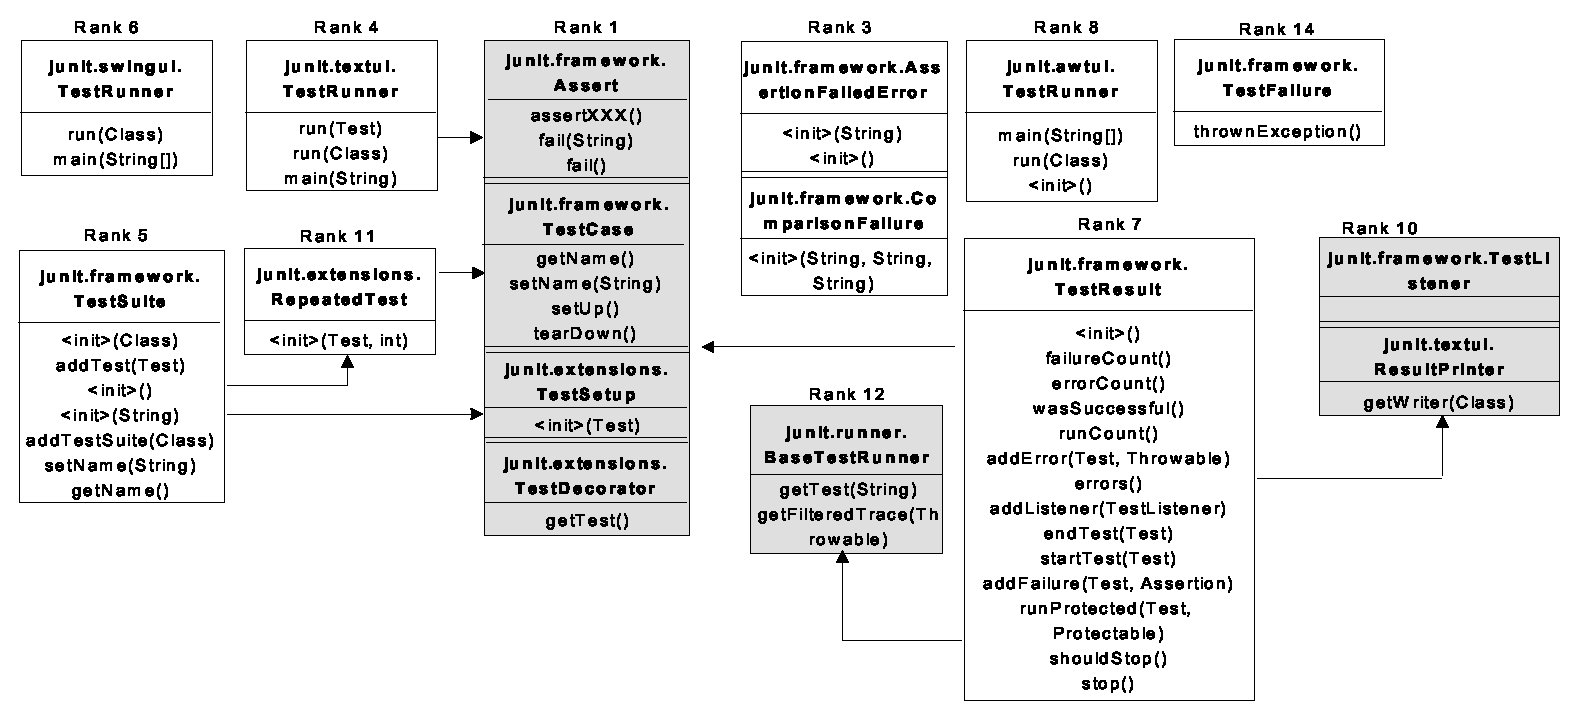
\includegraphics[scale=0.68,clip]{figs/examplehotspot_final.eps}
\caption{Hotspot hierarchies identified for the JUnit framework} \label{fig:hotspotexample}
\end{figure*}

We next use an example to explain our approach and show how the detected
hotspots and coldspots can be used by the framework users. We use JUnit~\cite{JUNIT}, the
\emph{de facto} standard unit testing framework for Java, 
as an illustrative example for explaining our approach.

SpotWeb accepts an input framework, say JUnit, and extracts
\emph{FrameworkInfo} from the framework. The
\emph{FrameworkInfo} includes all classes, all interfaces, public
or protected methods of each class and interface, and inheritance
hierarchy among classes or interfaces of the framework. SpotWeb also captures
the constants defined by the input framework. SpotWeb
constructs different queries for each class or interface and
interacts with a CSE such as Google code search~\cite{GCSE} to
gather relevant code examples from existing open source projects that
reuse the classes of the input framework. For example, SpotWeb constructs
a query such as ``\CodeIn{lang:java junit.framework.TestSuite}'' for
gathering relevant code examples of the \CodeIn{TestSuite} class. These
gathered code examples are referred as a \emph{LocalRepository} for
the input framework. SpotWeb analyzes gathered code examples
statically and computes \emph{UsageMetrics} for classes, interfaces,
and public or protected methods of all classes and interfaces. For
example, the \emph{UsageMetrics} computed for the \CodeIn{TestSuite}
class show that the class is instantiated for 165 times and is
extended for 32 times. Similarly, the \emph{UsageMetrics} computed
for the method \CodeIn{addTest} of the \CodeIn{TestSuite} class show
that the method is invoked for 95 times. SpotWeb also gathers code
examples for each class or method and stores these code examples in
a repository, referred as \emph{ExampleDB}. Then SpotWeb uses the
algorithm shown in Figure~\ref{alg:hotspotalgo} for detecting
hotspots from the computed \emph{UsageMetrics}.

Initially, SpotWeb ranks methods in a non-ascending order based on
their \emph{UsageMetrics} and uses a threshold percentage $HT$ to
detect hotspot methods: the methods in the top $HT$ percentage with
a non-zero \emph{UsageMetrics} are detected as hotspot methods. 
The detected hotspot methods are then
grouped into their declaring classes, detected as hotspot classes.
These hotspot classes are ranked based on the minimum rank of the
hotspot methods declared by these classes. SpotWeb classifies the
hotspot classes into two categories (templates and hooks) based on
heuristics described in Step 4 of the algorithm shown in Figure~\ref{alg:hotspotalgo}. The hotspot classes of each
category are further grouped into hierarchies based on their
inheritance relationships. For example, SpotWeb detected classes
\CodeIn{Assert} and \CodeIn{TestCase} as hook hotspots in the JUnit
framework. As \CodeIn{TestCase} class extends \CodeIn{Assert} class,
SpotWeb groups both the classes into the same hierarchy. SpotWeb
assigns a rank to each hierarchy based on the minimum rank of the
hotspot classes contained in the hierarchy. For example, consider
that the \CodeIn{Assert} class has Rank 1 and the \CodeIn{TestCase}
class has Rank 2, then the grouped hierarchy of the
\CodeIn{Assert} and \CodeIn{TestCase} classes is assigned with Rank
1. The rank attribute uniquely identifies a hierarchy among all
other hierarchies. Hierarchies with smaller ranks have higher preference
or importance to the hierarchies with larger ranks.

Figure~\ref{fig:hotspotexample} shows the hotspot hierarchies detected for the JUnit
framework. The figure also shows ranks assigned to each hierarchy.
As the rank attribute uniquely identifies a hierarchy, we use the
rank as an identity for describing a hierarchy.
Each hierarchy includes one or more hotspot classes and is shown as pairs of class and its methods.
For example, Hierarchy 1 (hierarchy with Rank 1) has classes \CodeIn{Assert}, \CodeIn{TestCase}, \CodeIn{TestSetup},
and \CodeIn{TestDecorator}. We show template hierarchies in white and hook hierarchies in gray.
For example, Hierarchy 1 is a hook hierarchy and Hierarchy 3 is a template hierarchy.

Methods inside each class of a hierarchy are sorted
based on their computed \emph{UsageMetrics}. Sorting methods of a class
can assist the framework users in quickly identifying the methods that are often
used inside a given hotspot class. For example, consider the \CodeIn{TestSuite} class
shown in Hierarchy 5. The \CodeIn{TestSuite} class has three constructors \CodeIn{<init>(Class)},
\CodeIn{<init>()}, and \CodeIn{<init>(String)}. However, the \CodeIn{<init>(Class)} constructor
is often used compared to the other two constructors. Due to space limit,
we show all assertion methods such as \CodeIn{assertEquals} and \CodeIn{assertTrue}
of the class \CodeIn{Assert} of Hierarchy 1 as \CodeIn{assertXXX}.

The figure also displays dependencies among hotspot hierarchies
(shown as arrows between hierarchies). SpotWeb captures the
usage relationships among hotspot classes through dependencies.
For example, Hierarchy $5$ has a
\CodeIn{TEMPLATE\_HOOK} dependency with Hierarchy $1$. This
dependency indicates that to reuse methods such as \CodeIn{addTest}
of the class \CodeIn{TestSuite} in Hierarchy 5, the user has to
define a new behavior for the classes in Hierarchy $1$.

\begin{figure}[t]
\begin{CodeOut}
\begin{alltt}
01:public class SRDAOTestCase 
02:\hspace*{0.4in}extends TestCase \{
03:\hspace*{0.1in}private SRDAO dao = null;...
04:\hspace*{0.1in}public SRDAOTestCase() \{
05:\hspace*{0.3in}super(); ... 
06:\hspace*{0.1in}\}
07:\hspace*{0.1in}protected void setUp() throws Exception \{
08:\hspace*{0.3in}...
09:\hspace*{0.3in}dao = (SRDAO)context.getBean("SRDAO");
10:\hspace*{0.3in}...
11:\hspace*{0.1in}\}
12:\hspace*{0.1in}public void tearDown() throws Exception \{
13:\hspace*{0.3in}dao = null; 
14:\hspace*{0.1in}\}
15:\hspace*{0.1in}public void testF() \{ ... \}
16:\hspace*{0.1in}public void testB() \{ ... \}
17:\hspace*{0.1in}...
18:\}
\end{alltt}
\end{CodeOut}
\Caption{\label{fig:hcodeexample} Suggested code example for the hook class \CodeIn{TestCase}.}
\begin{CodeOut}
\begin{alltt}
01:public class MyTestSuite \{ 
02:\hspace*{0.1in}...
03:\hspace*{0.1in}public static Test suite() \{
04:\hspace*{0.3in}TestSuite suite = new TestSuite("axis");
05:\hspace*{0.3in}suite.addTest(new SRDAOTestCase());
06:\hspace*{0.3in}return suite;
07:\hspace*{0.1in}\}
08:\hspace*{0.1in}...
09:\}
\end{alltt}
\end{CodeOut}
\Caption{\label{fig:tcodeexample} Suggested code example for the template class \CodeIn{TestSuite}.}
\end{figure}

We next describe how the hotspots detected by SpotWeb can be used by
the framework users to reuse classes of the JUnit framework. After reviewing
the hotspots shown in Figure~\ref{fig:hotspotexample}, consider that
a framework user wants to start with the method \CodeIn{addTest} of
the template class \CodeIn{TestSuite} in Hierarchy 5.
Figure~\ref{fig:hotspotexample} shows that Hierarchy 5 of the
\CodeIn{TestSuite} class has a \CodeIn{TEMPLATE\_HOOK} dependency
with the Hierarchy 1. This dependency indicates that the user may
need to define a new behavior for the associated hook hierarchy.
SpotWeb recommends the code example shown in
Figure~\ref{fig:hcodeexample} for the hook class \CodeIn{TestCase},
which is part of Hierarchy 1. The code example exhibits several
aspects that need to be handled by the user while extending the
\CodeIn{TestCase} class. For example, in the \CodeIn{setUp} method,
the user can write code for setting up the environment such as
instantiating necessary variables, and in the \CodeIn{tearDown}
method, the user can destroy the created variables. In addition, the code
example shows that names of the test methods in the extended class
of the \CodeIn{TestCase} class should start with the prefix \CodeIn{test}.
SpotWeb also recommends a code example for the \CodeIn{addTest} method and
the recommended code example is shown in
Figure~\ref{fig:tcodeexample}. The code example shows that the user
has to create an instance of the \CodeIn{TestSuite} class and then
add test cases through the \CodeIn{addTest} method.

An API class or method is identified as a coldspot if that class or method is neither
used directly nor used indirectly by gathered code examples. The complete
algorithm used for detecting coldspots is shown in Figure~\ref{alg:coldspotalg}. SpotWeb identified $20$
classes such as \CodeIn{Swapper}, \CodeIn{TestRunListener}, and \CodeIn{ExceptionTestCase} as coldspots
in the JUnit framework. However, coldspots are only suggestions
for users unfamiliar to that framework and SpotWeb does not intend to recommend users not to reuse
those coldspot classes. Sometimes, coldspots can also be helpful to
the framework developers in distributing their maintenance efforts, because the framework
developers can give a low preference to the coldspot classes.

%----------------------------------------------------------------------------------------------
%\section{Categorization of PUTs}
\label{sec:categorization}

We used suggested test patterns~\cite{halleux08:putpatterns} 
to generalize conventional unit tests. These test patterns can help developers in writing effective PUTs. Although PUTs alleviate the problem of writing different conventional unit tests to test the code under test with different input values, writing test oracles in PUTs could be a complex task. The developers are expected to specify sufficient assertions for testing various expected behaviors of executing the code under test. To deal with this complexity, developers can use test patterns to answer important questions of ``what'' scenarios of the code under test need to be tested and ``how'' they can be asserted. In our study, we found that a few test patterns are predominantly applicable while others are helpful in a few specific cases. 
In addition, we found that each PUT can be categorized into more than
one test pattern. In all, the patterns supported by Pex help write a wide range of PUTs for achieving high code coverage and reduce
PUT writing effort for both test-driven development and testing after the application is developed. 
We found that it was not easy to write PUTs for a few scenarios of the code under test using these patterns. To address this issue, we proposed two new patterns that can help in writing PUTs. We first explain the categories of the existing patterns as \textit{used} and \textit{not used} based on whether there are PUTs that belong to the test pattern and later present our proposed new patterns.
%---------------------------------------------------------------------------------------
\subsection{Existing Test Patterns}

We next present the classification of our PUTs into existing test patterns. Table~\ref{tab:patterns} shows the $15$ existing test patterns~\cite{halleux08:putpatterns}. Column 1 provides the classification of each pattern in our study. We put the existing test patterns into two categories based on their usage in this study: used and not used. Column 2 provides the pattern identifier. We use these identifiers to refer to the patterns in this section. Column 3 provides the pattern name and Column 4 gives the attributes\footnote{Pex provides a set of custom attributes to tag test class, test methods or parameters.} and methods supported by Pex for that pattern. 

\setlength{\tabcolsep}{2pt}
\begin{table*}[t]
\begin{center}
\centering \caption {\label{tab:patterns} Existing Test Patterns Supported By Pex.} \vspace*{0.1in}
\begin {tabular} {|l|r|l|l|}
\hline
Category					&	Pattern\#	&	Pattern Name												&	Pex Supported Attributes or Methods\\
\hline
Used							&	2.1				&	Arrange, Act, Assert								&	\\
\cline{2-4}
									& 2.2				&	Assume, Arrange, Act, Assert  			&	\\
\cline{2-4}
									&	2.3				&	Constructor Test										&	\\
\cline{2-4}
									& 2.4				&	Roundtrip														&	\\
\cline{2-4}
									& 2.5				&	Sanitized Roundtrip									&	\\
\cline{2-4}
									& 2.6				&	State Relation											&	\\
\cline{2-4}
									&	2.7				&	Same Observable Behavior						&	\\
\cline{2-4}
									&	2.8				&	Commutative Diagram									&	\\
\cline{2-4}
									& 2.9				&	Cases																&	PexAssert.Case() 			\\ 
\hline
Not used					& 2.10			&	Allowed Exception										&	[PexAllowedException]	\\
\cline{2-4}
									& 2.11			&	PexAllowedException									&	[PexExpectedGoals]		\\
\cline{2-4}
									&	2.12			&	Parameterized Stub									&	[PexAssumeUnderTest]	\\
\cline{2-4}
									&	2.13			&	Manual Output Review								&	PexStore.Value()			\\
\cline{2-4}
									&	2.14			&	Regression Tests										&	PexStore.ValueForValidation()\\
\cline{2-4}			
									& 2.15			&	Differential Regression Test Suite	&	\\
\hline
\end{tabular}
\end{center}
\end{table*}

\begin{enumerate}
\item \textbf{Used}: We put a pattern under this category if that
pattern was used at least once when writing PUTs.
We used 9 Patterns (from Pattern 2.1 to 2.9) for writing PUTs. Figure~\ref{fig:patterndistribution} shows the 
distribution of pattern usage across all the 70 PUTs. The x axis of the 
chart shows the used patterns and the y axis shows the number of PUTs that belong to each pattern.
For each test pattern, we show the number of PUTs in our study. 

\item \textbf{Not used}: We put a pattern under this category if that 
pattern was not used in test generalization. We found that $5$ 
out of the $15$ patterns were not used in writing PUTs in our study  
(from 2.10 to 2.15). The possible reason for not using these patterns 
in our test generalization is the lack of purposes for these patterns 
in our current study. For example, Patterns 2.14 and 2.15 are applied 
in the context of regression testing. However, in our current study, our
focus is not on regression testing. 
\end{enumerate}

\begin{figure}[t]
\centering
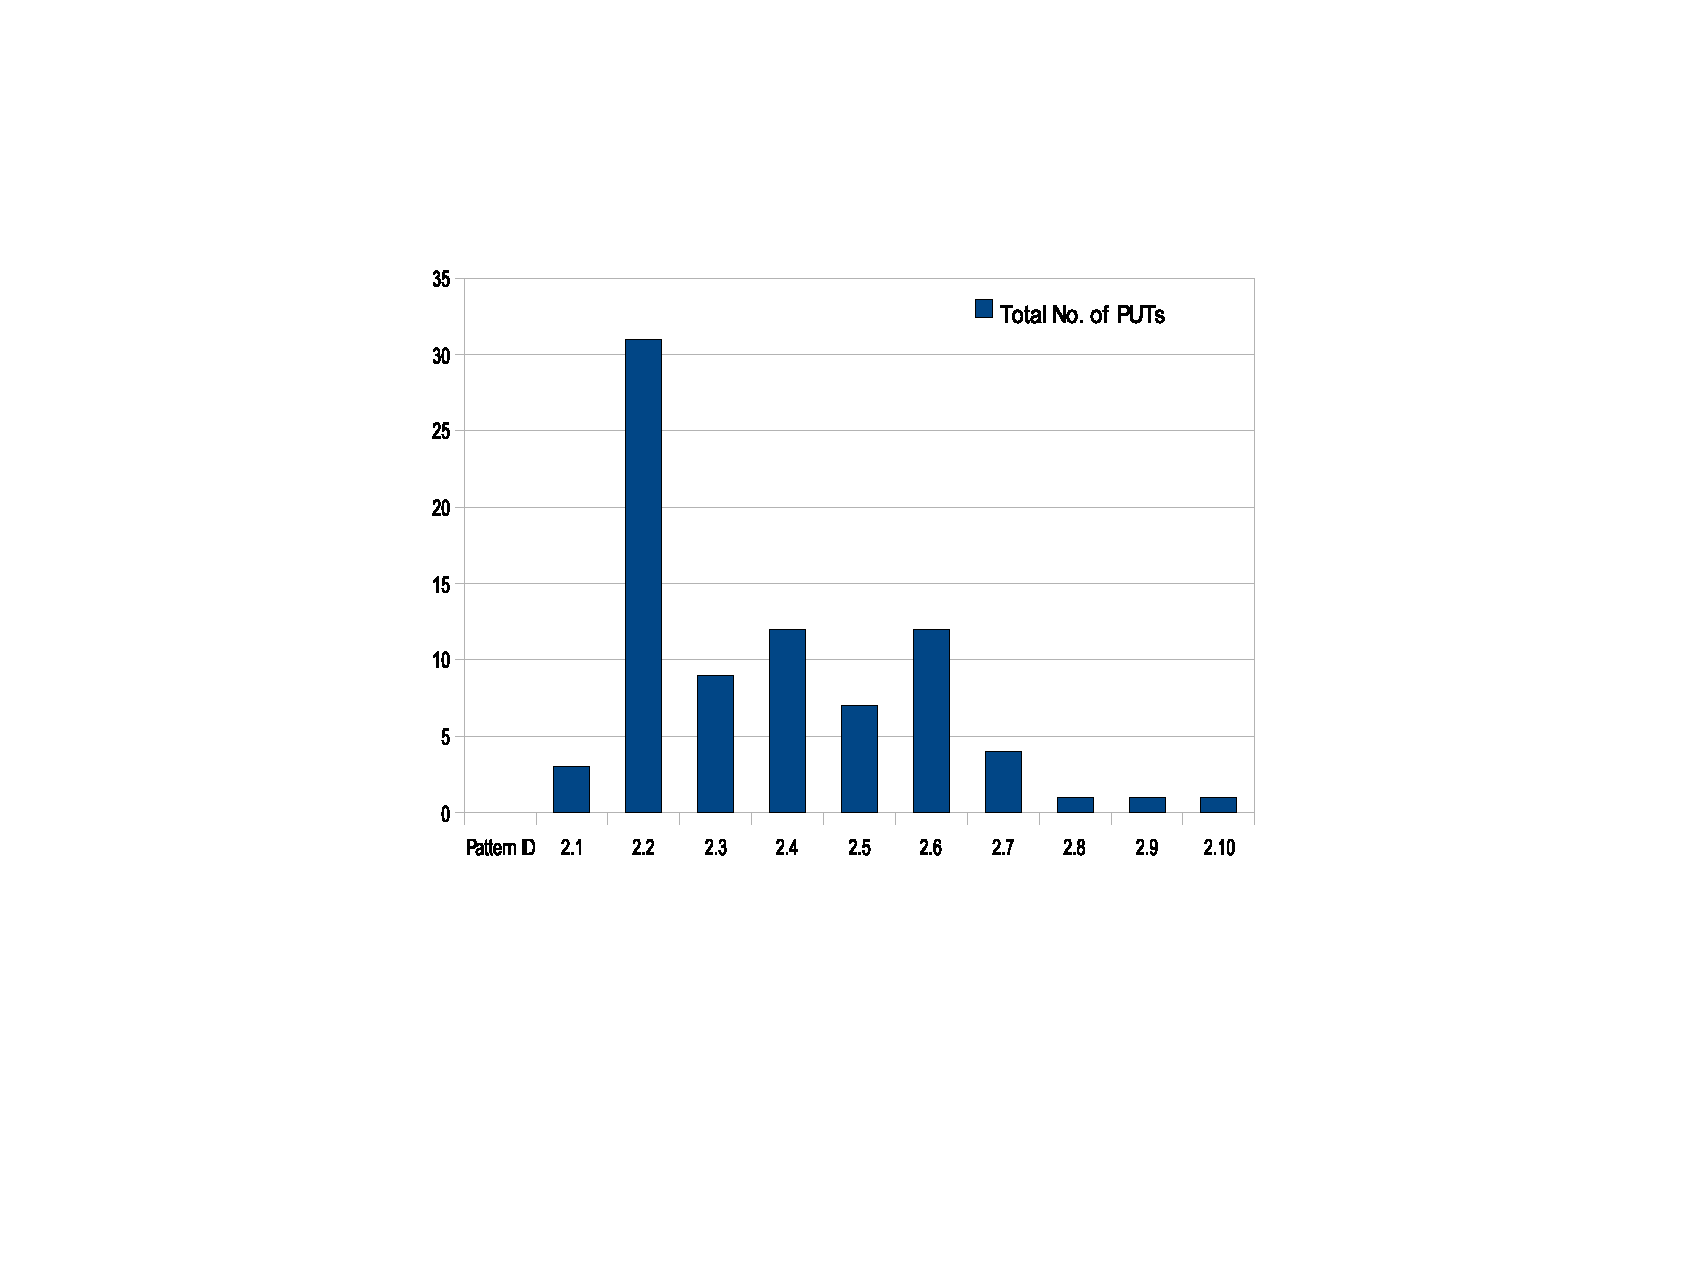
\includegraphics[scale=0.55,clip,trim=180 180 150 100]{figs/patterndistributionSeparated.eps}
\caption{\label{fig:patterndistribution}Distribution of test patterns for 70 PUTs. \textit{The distribution shows that in our testing, only patterns from 2.1 to 2.9 were used.}}
\end{figure}
%---------------------------------------------------------------------------------------
\subsection{New Patterns}
\label{sec:newpatterns}

We next describe two new patterns that can be supported, and that we found useful during our test generalization for the NUnit framework. 
%-------------------------------------------------------------------------------------------
\subsubsection{Random Selection of Cached Values}
\emph{Purpose}: To reuse generated values by maintaining a pool and randomly picking from those values.
\newline
\emph{Motivation}: We next show the motivation for such a pattern with an illustrative example. In the test generalization phase, we needed to generalize an existing unit test 
that requires to verify whether adding a \CodeIn{RegisterKey} to an \CodeIn{NUnitRegistry} and 
then clearing the \CodeIn{NUnitRegistry} work as expected. The \CodeIn{NUnitRegistry} class holds \CodeIn{RegisterKeys} as a tree structure with a main key and an unrestricted number of subkeys in a tree-structured form. Manually adding values and creating a tree structure to check both horizontal and vertical cases at the same time was possible in the existing conventional unit test. However, when the test was parameterized, we were able to write a PUT to add all \CodeIn{RegisterKeys} either to one main key or add each \CodeIn{RegisterKey} to the last added key. Due to such restriction, the unit tests generated by this PUT
resulted in a reduced block coverage when compared to the conventional unit test, although there are a number of tests generated for the PUT. The rationale is that the tests generated for the PUT are expected to generate
a tree structure of keys to achieve high code coverage. As the existing test 
patterns do not meet our current requirement, we proposed a new pattern
where we maintain a pool of existing \CodeIn{RegisterKeys} and randomly
select a key from this pool to add the newly created key as a subkey.
Our new pattern can help construct several forms of tree structures automatically.
Although we explain our motivation using the \CodeIn{RegisterKeys} test
example, our pattern is general and can be applied to tests that require
to reuse previously generated values.
\newline
\emph{Proposed Pattern}: When the input is of the type collection or an array and the values need to be reused by the code under test, 
the values generated by Pex can be added to a pool using our proposed method 
\CodeIn{PexStore.Pool(<name>,<value>)}. \CodeIn{PexStore.Pool()} method is expected to cache values (represented by \CodeIn{value}) for a particular variable (represented by \CodeIn{<name>}). Later, a value can be picked randomly from these cached values using another proposed method \CodeIn{PexStore.Pick(<name>)}. \CodeIn{PexStore.Pick()} method is expected to pick a value randomly from the cached store of the variable \CodeIn{<name>}. Figure~\ref{fig:treepattern} shows an application of our proposed pattern.

\begin{figure}[t]
\begin{CodeOut}
\begin{alltt}
00:[PexMethod()]
01:public void TestClearRoutinesPUT([PAUT]String[] key) \{
02:\hspace*{0.1in}PexAssume.IsTrue(key.Length > 1);
03:\hspace*{0.1in}for (int j = 0; j < key.Length; j++) \{
04:\hspace*{0.3in}PexAssume.IsNotNull(key[j]);
05:\hspace*{0.1in}\}
06:\hspace*{0.1in}NUnitRegistry.TestMode = true;
07:\hspace*{0.1in}using (RegistryKey mainKey = 
08:\hspace*{0.3in}NUnitRegistry.CurrentUser) \{
09:\hspace*{0.3in}//enabling appending values to a list
10:\hspace*{0.3in}\textbf{PexStore.Pool("keys",mainKey)}; 
11:\hspace*{0.3in}for (int j = 0; j < key.Length; j++) \{
12:\hspace*{0.5in}RegisterKey parentKey = 
13:\hspace*{0.7in}\textbf{PexStore.Pick("keys")} as RegisterKey;
14:\hspace*{0.5in}RegistryKey subKey = 
15:\hspace*{0.7in}mainKey.CreateSubKey(key[k - 1]);
16:\hspace*{0.5in}\textbf{PexStore.Pool("keys",subKey)};
17:\hspace*{0.3in}\}
18:\hspace*{0.3in}NUnitRegistry.ClearTestKeys();
19:\hspace*{0.3in}PexAssert.IsTrue(mainKey.SubKeyCount == 0);
20:\hspace*{0.1in}\}
21:\}
\end{alltt}
\end{CodeOut}
\Caption{A new test pattern that helps reuse previously generated values using a cache. \textit{The \CodeIn{PexStore.Pool()} method can be used to append the value \CodeIn{mainKey} to the cache of variable~\CodeIn{keys} and \CodeIn{PexStore.Pick()} method can be used to pick a random value from the cache of the variable \CodeIn{keys}}.}\label{fig:treepattern}
\end{figure}
%------------------------------------------------------------------------------------------------------------
\subsubsection{Unique-value generation}
\emph{Purpose}: To generate unique values when a parameter is a collection of values instead of a single value.
\newline
\emph{Motivation}: In our test generalization phase, for four PUTs, we were unable to achieve the same test effectiveness (i.e., block coverage) by the generated conventional unit tests as that of the existing unit tests. We found the reason to be a required object state: the required object state for the four PUTs to achieve high block coverage can be created only when a unique set of elements is available. For such PUTs, we had to write additional
code to ensure that Pex generates only unique values. For example, in the following PUT, we include a \CodeIn{for} loop with a \CodeIn{PexAssume} (as shown below) on each element of the collection to make sure that
Pex generates a set of unique values. 

\begin{CodeOut}
\begin{alltt}
//PAUT: PexAssumeUnderTest
01:public void SubstorageSettingsPUT1(
\hspace*{0.3in}[PAUT]String subName, [PAUT]String[] name)
02:\{
03:\hspace*{0.3in}PexAssume.IsNotNull(value); 
04:\hspace*{0.3in}PexAssume.IsTrue(name.Length == value.Length);
\hspace*{0.4in}/*assist Pex to generate unique values by 
							 **iterating over each array element and adding
							 **the assumption it is not equal to any other 
							 **array element*/
05:\hspace*{0.3in}for (int i = 0; i < name.Length; i++) \{
06:\hspace*{0.5in}for (int j = 0; j < name.Length; j++) \{
07:\hspace*{0.6in}PexAssume.IsFalse(name[i].Equals(name[j]));
08:\hspace*{0.5in}\}
09:\hspace*{0.3in}\}
10:\hspace*{0.1in}......
11:\}
\end{alltt}
\end{CodeOut}

\emph{Proposed Pattern}: When the input is of the type collection or an array, 
we propose a new pattern using a custom attribute called \CodeIn{PexGenerateUnique} that can inform
Pex to generate unique values. For example, applying the proposed pattern to the preceding example can
result in the following easy-to-write code. We also assume that 
\CodeIn{PexGenerateUnique} subsumes the properties of \CodeIn{PexAssumeUnderTest}.

\begin{CodeOut}
\begin{alltt}
//PAUT: PexAssumeUnderTest
01: public void SubstorageSettingsPUT1([PAUT]String 
\hspace*{0.3in}subName, [\textbf{PexGenerateUnique}]String[] name)
02:\{
03:\hspace*{0.3in}PexAssume.IsNotNull(value); 
04:\hspace*{0.3in}PexAssume.IsTrue(name.Length == value.Length);
05:\hspace*{0.1in}.....
06:\}
\end{alltt}
\end{CodeOut}

For the four PUTs that required generation of a set of unique values, we could apply the proposed pattern as shown in the preceding code example and achieve the test effectiveness.

%----------------------------------------------------------------------------------------------
%\section{Patterns and Supporting Techniques}
\label{sec:helper}

We next detail on the PUT patterns and supporting techniques that can be used in writing PUTs. In our study, we primarily use patterns to help generalize test oracles. In addition, we use the supporting techniques of factory methods and mock object to deal with the issues of desirable object states and interactions of the code under test with the environment, respectively. We next describe these techniques in detail.

%-------------------------------------------------------------------------
\subsection{PUT Patterns}
\label{sec:patterns}

A major challenge of writing PUTs is writing a generalized test oracle. When writing CUTs, it is not challenging to write test oracles since for a particular CUT, expected output values can be easily determined for the given input test data based on the method under test. In contrast, when testing with PUTs, determining the expected output values is not trivial; a PUT should be designed to assert output values based on a number of input values generated by Pex for that PUT. To address this issue, we propose $15$ PUT patterns~\cite{halleux08:putpatterns} that help developers to deal with this issue of generalizing test oracles. Table~\ref{tab:patterns} shows $13$ of the proposed $15$ PUT patterns\footnote{The other two PUT patterns are related to regression testing, which is not within the scope of our paper.}.

\setlength{\tabcolsep}{2pt}
\begin{table}[t]
\begin{center}
\begin {tabular} {|r|l|}
\hline
									\#			&	Pattern Name									\\				%&	Pex Supported Attributes or Methods\\
\hline
\hline
									1				&	Arrange, Act, Assert (AAA)					\\				%&	\\
\hline
									2				&	Assume, Arrange, Act, Assert (AAAA) 	\\			%&	\\
\hline
									3				&	Constructor Test							\\				%&	\\
\hline
									4				&	Roundtrip											\\				%&	\\
\hline
									5				&	Sanitized Roundtrip						\\				%&	\\
\hline
									6				&	State Relation								\\				%&	\\
\hline
									7				&	Same Observable Behavior			\\				%&	\\
\hline
									8				&	Commutative Diagram						\\					%&	\\
\hline
									9				&	Cases													\\					%&	PexAssert.Case() 			\\ 
\hline
									10			&	Allowed Exception							\\					%&	[PexAllowedException]	\\
\hline
									11			&	Reachability									\\					%&	[PexExpectedGoals]		\\
\hline
									12			&	Parameterized Stub						\\					%&	[PexAssumeUnderTest]	\\
\hline	
									13			&	Manual Output Review					\\					%&	PexObserve.Value			\\
\hline
%									14			&	Regression Tests							\\					%&	PexStore.ValueForValidation()\\
%\hline
%									15			&	Differential Regression Test Suite	\\%&	\\
%\hline
\end{tabular}
\caption {\label{tab:patterns} PUT Patterns}  \vspace*{-3ex}
\end{center}
\end{table}

The proposed PUT patterns serve two purposes: (1) they assist in designing a PUT based on the developers' test objective, and (2) they assist in determining test oracles that can deal with the generality of the PUT. Patterns 1, 2, 9, 10, and 11 (shown in Table~\ref{tab:patterns}) primarily assist developers in designing PUT based on the test objective. For example, developers can use Pattern 2 (AAAA) when the method under test needs to be tested for a particular range of input values (the PUT includes assumptions), and the behavior of the method under test can be asserted using assertion statements (the PUT includes assertions). Similarly, developers can use Pattern 10 (Allowed Exception) when a method under test may throw a particular exception, and such an exception being raised does not indicate that the unit test fails. 
The remaining patterns listed in the table assist developers in writing test oracles. For example, developers can use Pattern 6 (State Relation) when a method under test causes an internal change to the object state, which in turn can be observed through other methods. 

\begin{figure}
\begin{CodeOut}        
\begin{alltt}
01: public void Clear()
02: \{
03: \hspace{0.07in}root = null;
04: \hspace{0.07in}Count = 0;
05: \}
\end{alltt}        
\end{CodeOut}\vspace*{-4ex}
\caption{\CodeIn{Clear} method of \CodeIn{AvlTree} class of DSA.}
\label{fig:pattern}%

\begin{CodeOut}        
\begin{alltt}
01: public void ClearCUT()
02: \{
03: \hspace{0.07in}AvlTree<int> actual = new AvlTree<int> \{ 1,3,5,6,9,7 \};
04: \hspace{0.07in}Assert.AreEqual(6, actual.Count);
05: \hspace{0.07in}actual.Clear();
06: \hspace{0.07in}Assert.AreEqual(0, actual.Count);            
07: \}
\end{alltt}
\end{CodeOut}\vspace*{-4ex}
\caption{Existing CUT to test the \CodeIn{Clear} method.}%
\label{fig:patternCUT}%
\end{figure}

We next illustrate the use of PUT patterns in designing a PUT and in determining a test oracle. Figure~\ref{fig:pattern} shows the \CodeIn{Clear} method from \CodeIn{AvlTree} of the DSA~\cite{dsa} library. The \CodeIn{Clear} method clears the contents of the \CodeIn{AvlTree} object. Figure~\ref{fig:patternCUT} shows the existing CUT to test the \CodeIn{Clear} method. The objective of the CUT is to create an \CodeIn{AvlTree} object with the given list of items, invoke the \CodeIn{Clear} method, and assert if the elements are removed. To transform this CUT to a PUT, developers promote the input list to the constructor of \CodeIn{AvlTree} as a parameter to the PUT. Based on the test objective, developers identify two patterns to write the PUT: (1) AAAA, there should be an assumption on the parameter since the parameter should be non-null, and the result of the \CodeIn{Clear} method should be asserted, and (2) State Relation, since the behavior of the \CodeIn{Clear} method can be observed using the \CodeIn{Count} field, i.e., observe the change in the object state. Using the identified patterns, developers can write a PUT shown in Figure~\ref{fig:patternPUT}. 

\begin{figure}
\begin{CodeOut}        
\begin{alltt}
01: public void ClearPUT([PAUT]List<int> values)
02: \{
03: \hspace{0.07in}AvlTree<int> actual = new AvlTree<int>(values);
04: \hspace{0.07in}PexAssert.AreEqual(values.Count, actual.Count);
05: \hspace{0.07in}actual.Clear();
06: \hspace{0.07in}PexAssert.AreEqual(0, actual.Count);
07: \}
\end{alltt}
\end{CodeOut}\vspace*{-4ex}
\caption{PUT transformed from CUT in Figure~\ref{fig:patternCUT}, using the AAAA and State Relation patterns.}%
\label{fig:patternPUT}%
\end{figure}

%-------------------------------------------------------------------------
\subsection{Factory Methods}
\label{sec:factory}

Pex faces challenges in handling PUT parameters of non-primitive types, because these parameters require method-call sequences (that create and mutate objects of non-primitive types) to generate desirable object states. These desirable object states are the states that help explore new paths or branches in the code under test. For example, a desirable object state to cover the \CodeIn{true} branch of Statement 8 in Figure~\ref{fig:cut} is that the \CodeIn{storage} object should already include a value for the setting name \CodeIn{sn}. Although Pex includes a demand-driven strategy for generating method-call sequences, Pex's strategy can generate method-call sequences effectively in certain limited scenarios where the constructors either accept primitive parameters or explicitly state the actual type of the parameter.

To assist Pex in generating effective method-call sequences that can help achieve desirable object states, developers can write method-call sequences inside factory methods, supported by Pex. Figure~\ref{fig:factorymethd} shows an example factory method for the \CodeIn{MemorySettingsStorage} class. The factory method accepts two arrays of setting names (\CodeIn{sn}) and values (\CodeIn{sv}) and adds these entries to the storage. This factory method helps Pex to generate method-call sequences that can create desirable object states. For example, Pex can generate five names and five values as arguments to the factory method for creating a desirable object state with five elements in the storage\footnote{Note that the factory methods provide only an assistance to Pex in achieving the desirable object states, and Pex generates these object states based on the branching conditions in the code under test.}. The same factory method can be reused for all other PUTs using the \CodeIn{MemorySettingsStorage} class as parameter types.

%-------------------------------------------------------------------------
\subsection{Mock Objects} 
\label{sec:mock}

A mock object~\cite{mockobjects} is an implementation for simulating environments such as file systems. Mock objects help test unit behaviors in isolation where the interactions of the unit under test with the real environment are replaced with the mock objects. Automatic test generation tools such as Pex could require various desirable environment states to generate high-covering unit tests. Creating these desirable environment states requires extensive test setup. Since such test setup can generate a lot of garbage in the environment (such as adding extra files in the file system), a significant amount of test cleanup is also required. We next describe how developers can use mock objects with an example from our study. 

\begin{figure}
\begin{CodeOut}
\begin{alltt}
01: public class MockXmlTextWriter\{ 
02:\hspace*{0.1in}public MockXmlTextWriter(string filename,
\hspace*{0.25in} Encoding encoding)
03:\hspace*{0.1in}\{
04:\hspace*{0.3in}this.fileName = filename;
05:\hspace*{0.1in}\}

06:\hspace*{0.1in}public void WriteAttributeString
\hspace*{0.3in}(string attributeName, string value)
07:\hspace*{0.1in}\{
08:\hspace*{0.3in}xmlString = xmlString + " " + attributeName 
\hspace*{0.7in}+ "=" + "\"" + value + "\"";
09:\hspace*{0.1in}\}

10:\hspace*{0.1in}public void Close()
11:\hspace*{0.1in}\{
12:\hspace*{0.3in}xmlString = xmlString.Replace("/> />", "/>" + 
   \hspace*{0.5in}System.Environment.NewLine + "</" 
   \hspace*{0.7in}+ startString + ">");
13:\hspace*{0.3in}CreatedProjects.currentProject = xmlString;
14:\hspace*{0.1in}\}
\hspace*{0.3in}............
15: \}
\end{alltt}
\end{CodeOut}  \vspace*{-3ex}
\caption{\label{fig:mockobject} Sample code from the \CodeIn{MockXmlTextWriter} mock object. In the \CodeIn{WriteAttributeString} method, the argument string is appended to a global string \CodeIn{xmlString} and this global string represents the content written to the xml file.}  \vspace*{-3ex}
\end{figure}

In the \CodeIn{NUnitProject} class of the NUnit application, to test the \CodeIn{save} method, the developer can use a mock object to replace the interactions of code under test with the \CodeIn{XmlTextWriter}. The purpose of the \CodeIn{save} method is to write configuration information to an XML file. This XML file is expected to be created when the project is created, i.e., an instance of \CodeIn{NUnitProject} is created. Two existing CUTs \CodeIn{SaveEmptyConfigs} and \CodeIn{SaveNormalProject} test this \CodeIn{save} method. These CUTs add configurations to the XML project files and assert whether the files are saved in the right format and contain the added configuration information. Both the CUTs depend on a default empty project that is created using the test setup method. Therefore, the requirement to test the \CodeIn{save} method is to provide the project configuration file (the XML file) in a \emph{specific location}, i.e., the directory location where the project is saved (when a project is saved, a new directory is created as the project directory and the XML file is created in this directory). 

To generalize these CUTs, the developer can promote the project path (a parameter to the \CodeIn{save} method and a local variable in the CUTs) as a parameter to the PUT. However, generalization of these CUTs is not straightforward. By promoting the project path as the PUT's paramater, every unit test generated by Pex using the PUT requires an XML file in the location (reflected by the generated value for the parameter). The reason is that when the \CodeIn{save} method is invoked, the XML file is accessed using \CodeIn{XmlTextWriter}. Without the XML file, the \CodeIn{save} method throws an exception. Therefore, to avoid the complexity of creating a ``real'' file at a ``real'' location and to prevent the exception thrown by the \CodeIn{save} method, the developer can mock the expected behavior of \CodeIn{XmlTextWriter} with \CodeIn{MockXmlFileWriter}. This mock object simulates the behavior of \CodeIn{XmlTextWriter}, but unlike the real object, it appends the input text to a \CodeIn{string}, still preserving the output of the actual behavior of \CodeIn{XmlTextWriter}, and avoiding the interactions with the file system. Figure~\ref{fig:mockobject} shows a code snippet of the \CodeIn{MockXmlTextWriter} class. By using the mock-object technique, the developer can achieve generalization of both the CUTs to test the \CodeIn{save} method.

%The \CodeIn{xml} file was expected to already exist physically for the test to execute so that the code under test can access the file and add configuration information to the file, and test if the project is correctly saved with the configurations. The existing tests save the projects and assert by reading the \CodeIn{xml} file using a stream reader and check against an expected string (which is constructed based on the configurations that are added). 
%------------------------------------------------------------------------------------------------------

%\subsection{Input-Space Partitioning}
%\label{sec:inputspace}
%
%Input-space partitioning~\cite{paul:offut} helps partition the input space into disjoint blocks,
%where the union of all the blocks should result in the complete input space.  
%We explain how we performed the input-space partitioning in our study to achieve
%a higher coverage of the method \CodeIn{SaveSetting} of the class
%\CodeIn{SettingsGroup}. The \CodeIn{SaveSetting} method accepts an argument of type
%\CodeIn{Object}. The method accepts several types such as \CodeIn{int}, \CodeIn{string},
%\CodeIn{bool}, and \CodeIn{enum}, and a different path of the code is covered for each type. Therefore, in order to achieve high code coverage, a PUT to test this method should be designed to generate conventional unit tests that take different types of the argument. For simplicity, we explain how we dealt with
%integers and strings only. We defined two partitions where the first partition includes
%integers and the second partition includes strings. We wrote separate PUTs for
%covering these partitions. We repeated the same procedure for other input types. Consequently, Pex achieved high coverage as it was able to generate different input types and cover several program paths.
%----------------------------------------------------------------------------
%\subsection{Delegates} 
%\label{sec:delegate}
%
%Delegates are used to encapsulate a method with a specific signature and 
%a return type. These delegates are used to pass methods as arguments instead
%of data, which is commonly used in practice. Such a feature is quite helpful
%when the method to be called is known \emph{only} during runtime. These delegates
%feature is often used in GUI applications for event-handling. In our study, we found that some code portions are not covered as those portions require the delegates
%to be defined. We next show an example delegate class we used in Phase 2 of our study.
%% We expect that Pex can be easily extended to provide support for
%%delegates also. We next explain how Pex can be extended to provide such support
%%with illustrative examples. 
%\begin{figure}
%\begin{CodeOut}
%\begin{alltt}
%00:namespace Application \{
%01:\hspace*{0.1in}public delegate int MyHandler(object sender, 
%02:\hspace*{0.8in}MyEventArgs e);
%03:\hspace*{0.1in}class DelegateClass \{
%04:\hspace*{0.2in}public int DMethod(object sender, MyEventArgs e)\{
%05:\hspace*{0.3in}Console.WriteLine("In Delegate {0}", e.m_id);
%06:\hspace*{0.2in}\}
%07:\hspace*{0.2in}public A(TestCls b)\{
%08:\hspace*{0.3in}MyHandler d1 = new MyHandler(DMethod);
%09:\hspace*{0.3in}b.Event += d1;
%10:\hspace*{0.2in}\} 
%11:\hspace*{0.1in}\}
%12:\hspace*{0.1in}class TestCls \{
%13:\hspace*{0.2in}public event MyHandler Event;        
%14:\hspace*{0.2in}public void MUT(MyEventArgs e)\{
%15:\hspace*{0.3in}if (Event != null) \{
%16:\hspace*{0.4in}Event(this, e); \}
%17:\hspace*{0.3in}\}
%18:\hspace*{0.2in}\} 
%19:\hspace*{0.1in}\}
%20:\}
%\end{alltt}
%\end{CodeOut}
%\Caption{\label{fig:delegateex} A code example with a delegate handler.}
%\end{figure}
%
%Figure~\ref{fig:delegateex} shows two classes \CodeIn{DelegateClass}
%and \CodeIn{TestCls}. \CodeIn{TestCls} defines a method under test
%with the name \CodeIn{MUT}. When the method \CodeIn{MUT} is executed 
%without defining any delegate handler, Pex cannot cover Statement 16. 
%We manually created a delegate handler 
%with the name \CodeIn{DelegateClass} and added the handler using
%the operator \CodeIn{+=} as shown in Statement 9. These delegate handlers
%are different from normal method calls as there can be multiple delegate handlers
%that can be registered for one event. 
%Pex can be extended 
%to provide additional feature to automatically take care of
%delegate handlers. Pex can generate mock methods based on the signature
%of delegate (shown in Statement 1). For example, Pex can generate a
%mock method with argument types \CodeIn{object} and \CodeIn{MyEventArgs}
%with the following code inside the method.

%\begin{CodeOut}
%\begin{alltt}
%\hspace*{0.1in}var chooser = PexChoose.FromCall(this);
%\hspace*{0.1in}return chooser.ChooseResult<int>();
%\end{alltt}
%\end{CodeOut}

%The preceding method can replace the manually written delegate handler
%shown in Statements 3 to 11 in Figure~\ref{fig:delegateex}.
%The reason for using \CodeIn{PexChoose} in the automatically generated
%mock methods is that Pex can later infer the return value of the mocked
%delegate handler based on the further branch conditions in the source code.
%Sometimes, there can be more than one delegate handler associated with 
%each event such as the method call \CodeIn{Event} in Statement 16. Pex can
%simulate such behavior by defining multiple mock methods for
%each \CodeIn{Event}. One issue that can arise is that when there are multiple
%delegate methods for each \CodeIn{Event}, there can be multiple return values.
%In this scenario, C\# documentation suggests to use the return value
%that is returned from the last delegate.
%----------------------------------------------------------------------------------------------
%\section{Benefits of PUTs}
\label{sec:newbenefits}
We next present the benefits of retrofitting conventional unit tests for PUTs. 
In test generalization, we transformed 57 conventional unit tests of 10 test classes resulting in 49 PUTs.  In order to achieve higher block coverage, we wrote 21 new PUTs for 6 of the 10 classes under study. Table~\ref{tab:oldbenefits} shows the results of writing PUTs. Column ``Test Class'' shows the names of the test class and Column ``Test Methods'' shows the statistics of existing 
conventional test methods, the test methods that are amenable to 
test generalization, the percentage of amenable conventional unit tests, the number of transformed PUTs, and the number of new PUTs that were written. The five sub-columns 
represented by ``Conventional'', ``\#Amenable'', ``\%'', ``\#PUT'', and ``\#New PUT'' give cumulative figures for all test methods in the corresponding class. ``\#PUT'' shows the number of PUTs written in Phase 1 and ``\#New PUT'' shows the number of new PUTs written in Phase 2 to achieve higher coverage. Section~\ref{sec:notamenable} provides details of the test methods that are not amenable to test generalization with illustrative examples. 
Column ``\% Coverage'' shows the block coverage reported by Pex on executing
tests. These two sub-columns show the average of all the test methods in each class. Column ``Avg. New Blocks'' 
shows the average number of new blocks covered by PUTs. As PUTs can verify more general behavior,
we found that PUTs achieve a high block coverage and cover new blocks
that are not covered by conventional unit tests. Column ``\#Defects'' shows the number of defects that were detected by the PUTs 
and were not detected by the existing conventional unit tests. 
This column again shows a cumulative value of all the test methods in a test class.
%---------------------NEW TABLE SHOWING THE BENEFITS OF TEST GENERALIZATION-----------------------
\setlength{\tabcolsep}{2pt}
\begin{table*}[t]
\begin{center}
\centering \caption {\label{tab:oldbenefits} Benefits of Retrofitting PUTs in Unit Testing} \vspace*{0.1in}
\begin {tabular} {|l|r|r|r|r|r|r|r|r|r|r|}
\hline
Test Class						&\multicolumn{5}{|c|}{Test Methods}				& \multicolumn{3}{|c|}{\% Coverage}						&Avg. New	&\#Defects\\
								 			&\multicolumn{5}{|c|}{}										&	\multicolumn{3}{|c|}{}											&Blocks		&\\
\cline{2-9}
											&\#Conventional	&\#Amenable		&\%					&\#PUT		&\#New PUT		&Conventional	&PUT		&With			&		&\\
											&								&							&						&					&							&							&				&New PUT	&		&\\
\hline
NUnitProjectSave.cs		&3							&1						&33.33			&1				&2						&35.71				&40.98	&57.91		&10		&0\\
\hline
NUnitRegistryTests.cs	&5							&5						&100.00			&4				&							&58.97				&72.80	&100.00		&0		&1\\
\hline
TestAgentTests.cs			&2							&2						&100.00			&2				&1						&100.00				&100.00	&NA				&0		&0\\
\hline
RegistrySettings-			&								&							&						&					&							&							&				&					&			&	\\
StorageTests.cs				&6							&5						&83.33			&6				&4						&45.34				&90.60	&100.00		&0		&1\\
\hline
MemorySettings-				&								&							&						&					&							&							&				&					&			&	\\
StorageTests.cs				&6							&4						&66.67			&4				&							&100.00				&100.00	&NA				&2		&0\\
\hline
PathUtilTests.cs			&7							&3						&42.86			&6				&							&85.00				&85.00	&NA				&0		&3\\
\hline
RecentFilesTests.cs		&22							&21						&95.45			&5				&6						&59.94				&76.08	&84.17		&14		&0\\
\hline	
ServerUtilityTests.cs	&2							&2						&100.00			&3				&1						&90.32				&90.32	&95.16		&0		&2\\
\hline
SettingsGroupTests.cs	&5							&5						&100.00			&6				&7						&66.94				&90.95	&94.13		&2		&0\\
\hline
ProcessRunnerTests.cs	&0							&NA						&NA					&NA				&NA						&NA						&NA				&NA			&NA		&NA\\
\hline
\end{tabular}
\end{center}
\end{table*}
%-------------------------------------------------------------------

The benefits discussed here primarily reflect the results of the test generalization phase as we compare the benefits of PUTs over the existing conventional unit tests. Section~\ref{sec:limitations} discusses the amount of effort we took in writing the new PUTs in comparison to generalizing the existing conventional unit tests. We found three major benefits of retrofitting conventional unit tests for PUTs: higher code coverage, detection of new defects, and reduced test code. We observed that generalization
increases code coverage and detected new defects that were not
detected by the existing conventional unit tests. 
We also identified that
a single PUT often helps to replace multiple conventional unit tests,
thereby reducing the amount of test code (as shown by Column ``\#Convention'' and Column ``\#PUT'' in Table~\ref{tab:oldbenefits}). Sections~\ref{sec:coverage}, \ref{sec:defects}, and \ref{sec:testcode} explain these details.
%-------------------------------------------------------------------
\subsection{Coverage}
\label{sec:coverage}

As generalized tests often help cover more scenarios, we found that
test generalization helped to have an effective increase in the block coverage as shown in Table~\ref{tab:oldbenefits}.
For example, test generalization of the \CodeIn{RegistrySettingsStorage}
class shows an increase in the coverage of 45.24\%.
In addition, the tests generated for the PUTs in the test generalization achieved coverage
of new blocks that are not covered by the existing conventional 
unit tests. In order to achieve more code coverage, we wrote 21 new PUTs for 6 classes and obtained an average increase of $35$\% code coverage (considering only those classes for which we wrote new PUTs).
%For example, the generalization of conventional
%unit tests in the \CodeIn{RecentFilesTests.cs} covered $14$
%additional blocks (on average for all PUTs). In one scenario of \CodeIn{RecentFilesTest.cs}, there is a decrease in the \% of coverage when the conventional unit tests were transformed to PUTs; however, there is a significant increase in the number of blocks covered by the PUTs. The decrease in the coverage is due to the increase in the number of blocks covered by the PUT when compared to the corresponding conventional unit-test. The difference is primarily due to the
%Pex strategy of reporting block coverage as Pex cannot detect the total number of blocks correctly
%when some methods are not analyzed. For example, the numbers of blocks covered by two PUTs in the \CodeIn{RecentFilesTest.cs} were 56 and 58, while the conventional unit tests accounted for 23 and 25, respectively. The ratio of blocks covered to the total number of blocks accounted by PUTs are 41/56 (73.21\%) and 41/58 (70.69\%). Similarly, for conventional unit tests the ratio was 18/23 (78.26\%) and 18/25 (72.00\%). Therefore, despite an increase in the total number of blocks covered, there is a decrease in the \% of code coverage. 
%Benefits of adding new PUTs was not only an increase in the code coverage, but also we were able to write new PUTs for three conventional unit tests, which were not amenable to test generalization.
%-------------------------------------------------------------------
\subsection{Defects}
\label{sec:defects}

After test generalization we found 7 new defects that were not detected by
the existing conventional unit tests. We next explain a defect detected 
by our test generalization. The \CodeIn{NUnitRegistry} 
class stores the \CodeIn{RegistryKeys} in a tree-structured hierarchy. 
For building the key hierarchy, a default key is taken as a main 
key and the given keys are added as sub-keys to the main key or to the other sub-keys. During testing, adding a key hierarchy and on checking for the count or on clearing the keys, we found abnormal behavior for two tests. The PUT was written to take three test inputs. For one of the tests generated by Pex, the test inputs were \CodeIn{t}, \CodeIn{t}, and \CodeIn{t}, and the other test case took the test inputs as \CodeIn{$\backslash$0}, \CodeIn{$\backslash$0}, and \CodeIn{$\backslash$0}. For the first test case, when the three inputs were added to a main key (two as sub-keys and the other as a sub-key to one of the added subkeys), the count check for the keys passed, i.e., \CodeIn{PexAssert(2, mainKey.SubKeyCount)} passed. The same assertion failed for the second case (with test inputs ``$\backslash$0'') with an assertion failure message, ``expected 2, got 1''. This defect shows that the failure was possibly due to missing check on invalid characters. 
%-------------------------------------------------------------------
\subsection{Test Code}
\label{sec:testcode}

Test generalization also helped reduce the 
test code as shown in Column ``\#PUT'' of Table~\ref{tab:oldbenefits}. Often, test
generalization either helps reduce the amount of code in a single test method or
helps combine multiple test methods into a single PUT. Figure~\ref{fig:caseput}
shows an example PUT of the pattern type \emph{Cases} that combined five conventional unit tests. Each conventional
unit test verifies one case in the corresponding PUT. In addition, the PUT achieved higher coverage compared
to the five conventional unit tests as the \CodeIn{MaxValue} is now accepted
as an argument and the concrete values are generated from the argument
based on captured constraints.

\begin{figure}[t]
\begin{CodeOut}
\begin{alltt}
[PexMethod]
public void CountOverOrAtMaxPUT1(int MaxValue) \{
\hspace*{0.1in}recentFiles.MaxFiles = MaxValue;
\hspace*{0.1in}PexAssert
\hspace*{0.2in}.Case(MaxValue < MIN)
\hspace*{0.3in}.Implies(() => MIN == recentFiles.MaxFiles)
\hspace*{0.2in}.Case(MaxValue == MIN)
\hspace*{0.3in}.Implies(() => MaxValue == recentFiles.MaxFiles)
\hspace*{0.2in}.Case(MaxValue > MIN && MaxValue < MAX)
\hspace*{0.3in}.Implies(() => MaxValue == recentFiles.MaxFiles)
\hspace*{0.2in}.Case(MaxValue == MAX)
\hspace*{0.3in}.Implies(() => MaxValue == recentFiles.MaxFiles)
\hspace*{0.2in}.Case(MaxValue > MAX)
\hspace*{0.3in}.Implies(() => MAX == recentFiles.MaxFiles);            
\} 
\end{alltt}
\end{CodeOut}
\Caption{\label{fig:caseput} Single PUT constructed from five conventional tests.}
\end{figure}

%----------------------------------------------------------------------------------------------
%\section{Conventional Unit Tests Not Am- enable to Test Generalization} 
\label{sec:notamenable}

In our study, we found that $12.75$\% of conventional unit tests are not amenable to test generalization. There are two common cases under which we found that conventional unit tests are not amenable to test generalization. 

\textbf{Default checks.} We found that there are multiple conventional unit
tests that verify default values, which are often static values. We suspect
that the purpose of these tests could be to make sure that the developers do not
change the static values accidentally. We suspect that these tests are
not amenable for test generalization as values verified by these tests
are constants.

\textbf{Missing test oracles.} We found that test generalization
may cause the loss of test oracles in some cases. These cases can often occur when generalizing conventional unit tests that belong to the PUT patterns \emph{Roundtrip} and \emph{Commutative diagram}.
We explain this issue using the illustrative example shown below.

\begin{CodeOut}
\begin{alltt}
public void Canonicalize() \{
\hspace*{0.1in}PexAssert.AreEqual(@"C:/folder1/file.tmp",
\hspace*{0.3in}PathUtils.Canonicalize(@"C:/folder1/./folder2/
\hspace*{0.3in}../file.tmp")); 
\}
\end{alltt}
\end{CodeOut}
 
The \CodeIn{Canonicalize} method in \CodeIn{PathUtils} accepts
a \CodeIn{string} parameter and uses a complex procedure to transform the input \CodeIn{string} into a standard form. It is easy to identify the expected output for concrete strings
such as ``\CodeIn{C:/folder1/.../folder2/.. ./file.tmp}''. However, when the
conventional unit test is generalized with a parameter for the input string, it is challenging to 
identify the expected output. Developers need to implement a logic to assert the behavior of the method under test. The amount of effort required in such cases could be higher than the effort required to write the implementation of the actual method under test and therefore such conventional unit tests are not amenable to test generalization.

%----------------------------------------------------------------------------------------------
%\section{Discussion} 
\label{sec:limitations}

In our empirical study, we identify that it is difficult to generalize test oracles in a few cases. For example, consider the following CUT:\vspace*{-1.5ex}

\begin{CodeOut}
\begin{alltt}
public void Canonicalize() \{
\hspace*{0.1in}PexAssert.AreEqual(@"C:/folder1/file.tmp",
\hspace*{0.3in}PathUtils.Canonicalize(@"C:/folder1/./folder2/
\hspace*{0.3in}../file.tmp")); 
\}
\end{alltt}
\end{CodeOut} \vspace*{-1.5ex}

\noindent The \CodeIn{Canonicalize} method in \CodeIn{PathUtils} accepts a \CodeIn{string} parameter and uses a complex procedure to transform the input into a standard form. It is easy to identify the expected output for concrete strings such as \CodeIn{C:/folder1/.../folder2/.../file.tmp}. However, when the CUT is generalized with a parameter for the input string, it is challenging to identify the expected output. Although the developer can use our commutative diagram pattern and provide an alternative implementation for the \CodeIn{Canonicalize} method, the amount of effort required could be higher than the effort required to write the implementation of the actual method under test. In our empirical study, we still generalize these CUTs but do not generalize the test assertions, rather replace assertions with statements that print outputs suitable for manual review, i.e., use the Manual Output Review pattern of our proposed patterns. These PUTs can still help in detecting defects related to exceptions.

In our results related to the test code maintenance, there are a few cases where the number of PUTs are more than the number of CUTs. The reason is that Pex is not able to generate any CUT from the transformed PUT as Pex reached boundary values such as maximum number of branches exceeded. Although we tried to set higher boundary values, Pex is still not able to generate CUTs from those PUTs. Therefore, we performed a partial generalization by splitting the CUT into multiple PUTs.

We conducted our empirical study as third-party testers since we do not have the knowledge of the subject applications. We expect that our test generalization results can be much better if the test generalization is performed by the developers of these subject applications. The reason is that developers can incorporate their domain knowledge during test generalization to write more effective PUTs.

%One of the major limitations of PUTs is that PUTs requires more effort from developers than writing conventional unit tests requires. Although PUTs reduce the complexity of writing multiple conventional unit tests with various concrete test inputs, developers need additional expertise in writing such PUTs as PUTs are more generic compared to conventional unit tests. For example, writing PUTs requires developers to prescribe a test oracle that can deal with the generality of test inputs. We show that to reduce the complexity of writing PUTs, we adopted a methodology of writing PUTs in two phases. In Phase 1, we generalized the existing conventional unit tests to PUTs using suggested test patterns. In Phase 2, we used supporting techniques to write more PUTs to assist Pex in generating high-covering tests. 

%In our study, we observed that we took longer time to write PUTs in Phase 2 compared to the time we took in Phase 1. In Phase 1, we transformed the existing conventional unit tests to PUTs and the existing unit tests assist in writing PUTs as shown in Section~\ref{sec:example} with an example. In Phase 2, we discovered the un-covered code portions and wrote more PUTs to assist Pex to generate tests to cover the un-covered code portions. Based on our experience, we believe that to enjoy the test effectiveness achieved by writing PUTs and to reduce the cost involved in writing PUTs, a practical solution could be retrofitting PUTs by transforming these conventional unit tests to PUTs. We expect that writing a single conventional unit test to test a method under test and then transforming it to a PUT can help developers in writing the PUTs. Such a single conventional unit test can act as an \textit{example} unit test representing the intention of ``what'' needs to be tested. We expect that this methodology can both ease the process of writing PUT and still achieve high test effectiveness in unit testing. 

%As shown in our study, although the usage of the suggested test patterns and the supporting techniques can reduce effort of developers in writing PUTs and allow the test generation tool to generate high-covering tests, the complexity lies in being able to use them. In general, developers might consider it a tougher job to learn the supporting techniques and use them to write PUTs than writing multiple possible conventional unit tests. Nevertheless, our study shows that PUTs are more effective than conventional unit tests in detecting defects and also in achieving high code coverage. Therefore, we believe that the choice of writing PUTs is a trade-off between cost and benefit.
%----------------------------------------------------------------------------------------------
%\section{Related Work}
\label{sec:related}

Our approach is related to previous work on two areas:
language translation and library migration.

\textbf{Language translation.} To reduce manual efforts of language
translation~\cite{samet1981experience}, researchers proposed various
approaches~\cite{hassan2005lightweight,van1999identifying,waters1988program,mossienko2003automated,yasumatsu1995spice} to automate the process.
However, all these approaches focus on the syntax or structural differences between
languages. Deursen \emph{et al.}~\cite{van1999identifying} proposed an approach to identify
objects in legacy code. Their approach uses these objects to deal with the
differences between object-oriented and procedural languages. As
shown in El-Ramly \emph{et al.}~\cite{el2006experiment}'s experience
report, existing approaches support only a subset of APIs for language translation,
making the task of language translation a challenging problem.
In contrast to previous approaches, our approach automatically mines API mapping between
languages to aid language translation, addressing a significant
problem not addressed by the previous approaches and complementing
these approaches.

\textbf{Library migration.} With evolution of libraries, some APIs
may become incompatible across library versions. To address this
problem, Henkel and Diwan~\cite{henkel2005catchup} proposed an approach that captures
and replays API refactoring actions to update the client code.
Xing and Stroulia~\cite{xing2007api} proposed an approach that
recognizes the changes of APIs by comparing the differences between two
versions of libraries. Balaban \emph{et al.}~\cite{balaban2005refactoring} proposed
an approach to translate client code when mapping relations of libraries are
available. In contrast to these approaches, our approach focuses on
mapping relations of APIs across different languages. In addition, since
our approach uses ATGs to mine API mapping relations, our approach can also
mine mapping relations between API methods with different parameters or between
API methods whose functionalities are split among several API methods in the other language.

\textbf{Mining specifications.} Some of our previous approaches~\cite{zhong09:inferring,zhong09:mapo,thummalapenta09:mining,thummalapenta09:mseqgen,acharya09:mining} focus on mining specifications. MAM mines API mapping relations across different languages for language migration, whereas the previous approaches mine API properties of a single language to detect defects or to assist programming.

%----------------------------------------------------------------------------------------------
%\section{Threats to validity}
\label{sec:tov}
\vspace*{2ex}
The threats to external validity primarily include the degree to which the subject programs, faults, and conventional unit tests are representative of true practice. The number of classes used in our empirical study is relatively small, although the defects detected during our study are real defects. These threats could be reduced by conducting more studies with wider types of subjects in our future work. The threats to internal validity are due to manual process involved in writing PUTs. Our study results can be biased based on our experience and knowledge of the subject programs. These threats can be reduced by conducting more case studies with more subject programs and other human subjects. The results in our study can also vary based on other factors such as the effectiveness of our written PUTs and test generation capability of Pex. One threat to construct validity is that our study uses the block coverage reports generated by Pex to reflect the quality of tests.
%----------------------------------------------------------------------------------------------
%\section{Conclusion}
\label{sec:conclusion}

API Mapping relations serve as a basis for automatic translation tools to translate applications from one language to another. However, original and translated applications can exhibit different behaviors due to inconsistencies among mapping relations. In this paper, we proposed an approach, called TeMaAPI, that detects different behaviors of mapped API methods via testing. TeMaAPI targets at generating test cases that covers all feasible paths and  sequences to reveal different behaviors of both single methods and method sequences. We implemented a tool and conducted three evaluations on five translation tools to show the effectiveness of our approach. The results show that our approach detects various differences between mapped API methods. We further analyze these differences and their implications. We expect that our results can help improve existing translation tools and help programmers better understand differences of Java and C\#.

%Mapping relations of APIs are quite useful for the migration tools, but these mapping relations also can introduce defects to translated code since mapped API methods may have different behaviors. In this paper, we propose an approach, called TeMaAPI, that detects different behaviors of mapped API methods via testing. TeMaAPI targets at generating test cases that covers all feasible paths and  sequences to reveal different behaviors of both single invocations and invocation sequences. We implemented a tool and conducted three evaluations on five migration tools to show the effectiveness of our approach. The results show that our approach detects various differences between mapped API invocations. We further analyze these differences and their implications. The results can help improve existing migration tools and help programmers better understand differences of Java and C\#.

%----------------------------------------------------------------------------------------------
\begin{table*}[t]%
\centering
\begin{minipage}{\textwidth}
\centering
\begin{tabular}{|l|r|r|r|r|r|r|r|r|}
%----------------- HEADER ------------------------
\hline
Subject 		& Downloads 	& \multicolumn{4}{|c|}{Code Under Test} 					&	\multicolumn{3}{|c|}{Existing Test Code} \\ \cline{3-9}
						& 						&	\#Classes	&	\#Methods	& \#LOC	& Avg. Complexity	&	\#Classes	&	\#Methods &	\#LOC		\\ \hline\hline
%----------------- END HEADER ------------------------ 
NUnit				&		$193,563$\footnote{Anonymous read count in the year 2009}
													&						&						&				&									&						&						&					\\ \hline
DSA					&		$2241$		&						&						&				&									&						&						&					\\ \hline		
QuickGraph	&		$7969$ 		&						&						&				&									&						&						&					\\ \hline
\end{tabular}
%\footnotetext[1]{Anonymous read count in the year 2009}
\end{minipage}
\caption{Details of the subject applications}
\label{tab:subjectmetrics}
\end{table*}

\section{Empirical Study}

We conducted an empirical study using three real world applications to study the benefits of Parameterized Unit Tests (PUT) over Conventional Unit Tests (CUT) in specific and to show the applicability of the proposed systematic procedure in general. In our empirical study, we show the benefits of PUTs over existing CUTs in terms of three metrics: code coverage, defects, and test code maintenance. In particular, we address the following three research questions through our empirical study:

\begin{itemize}
	\item \textbf{RQ1: Coverage.} How much higher percentage of \emph{code coverage} is achieved by PUTs compared to existing CUTs? Since PUTs are a generalized form of CUTs, this research question helps to address whether PUTs can achieve additional coverage compared to CUTs.
	\item \textbf{RQ2: Defects.} How many new \emph{defects} (that are not detected by CUTs) are detected by PUTs and vice-versa? This research question helps to address whether PUTs have more fault-detection capabilities compared to CUTs.
	\item \textbf{RQ3: Test code maintenance.} How many number of tests are reduced by generalizing CUTs to PUTs? This research question helps to address whether PUTs require lesser efforts for maintaining test code compared to CUTs.
\end{itemize}

To address these research questions, we execute the existings CUTs of each application and execute the unit tests generated by Pex with the help of the transformed PUTs and measure the three metrics. Initially, we execute the existing CUTs and meticulously record the code coverage achieved and note the failing test cases as defects. In addition to that, we measure the number of CUTs and lines of code of each of the CUTs. We then generalize these CUTs to PUTs based on our systematic procedure. Consequently, we apply Pex using the generalized PUTs and record the coverage achieved, the number of failing test cases, the number of PUTs, and the number of lines of these PUTs. Furthermore, we manually analyze to ensure that the failing test cases did not fail due to invalid PUTs, such as missing assumptions on the parameters. We thus confirm that the test cases failed due to a defect in the code under test. \\

\noindent\textbf{Metrics.}
For our study, we measure two major metrics, (1) Branch coverage (2) Code metrics such as LOC and code complexity. For measuring the branch coverage of the code under test, we use a coverage measurement tool called NCover\footnote{http://www.ncover.com/}. For measuring the code metrics such as LOC and code complexity, we use the Count Lines of Code\footnote{http://cloc.sourceforge.net/} (CLOC) tool.

\subsection{Subject Applications}

We chose three open source applications to carry out our study, NUnit~\cite{nunit}, DSA~\cite{dsa}, and Quickgraph~\cite{quickgraph}. The criteria for choosing these projects are (1) large usage of the application in terms of the download records shown by the hosting site, (2) Existing conventional unit test suite size, (3) the size of the application sources, and (4) the code under test should contain non-trivial logic to validate the feasibility of test generalization. Table~\ref{tab:subjectmetrics} shows the characteristics of the three subject applications. Column ``Subject'' gives the name of the subject applications and Column ``Downloads'' gives the number of downloads of the applications as listed on the respective hosting websites. Column ``Code Under Test'' gives details of the code under test in the corresponding application in terms of the number of classes (``\#Classes''), number of methods (``\#Methods''), number lines of code (``\#LOC''), and the average complexity of the code under test. Column ``Existing Test Code'' provides details on the existing test code corresponding to the code under test. Subcolumns ``\#Classes'', ``\#Methods'', and ``\#LOC'' give the corresponding test code's metrics. In the following sections, we provide details on each of the subject applications.

\subsubsection{NUnit}
\label{sec:nunit}
We use an open source application, called NUnit~\cite{nunit}, as one of the subject applications for our study. NUnit, a counterpart of JUnit for Java~\cite{JUnit}, is a widely used open source unit-testing framework for all .NET languages. NUnit is written in C\# and uses attribute-based programming model~\cite{TDD} through a variety of attributes such as \CodeIn{[TestFixture]} and \CodeIn{[Test]}. The rationale behind choosing NUnit for test generalization is its popularity in terms of the number of downloads ($450$ anonymous reads in the year 2002 and $193,563$ in the year $2009$) of the application as listed by its hosting website SourceForge\footnote{http://sourceforge.net/}. Furthermore, the large number of manually written unit tests available with the project makes NUnit a good subject for test generalization. For the purpose of the study, we used $9$ classes from the \CodeIn{util} package (\CodeIn{nunit.util.dll}), which is one of the core components of the framework. We chose the \CodeIn{util} package in the study for two reasons: (1) it is one of the basic modules to be developed for the framework (2) it is an independent module and is not dependent on the other modules of the NUnit framework. We chose the $9$ classes as the code under test since the logic in these classes is non-trivial; the average complexity is $0$ as shown in Table~\ref{tab:subjectmetrics}. For our study, we used NUnit release version $2.4.8$. 

\subsubsection{DSA}

Data Structures and Algorithms (DSA)~\cite{dsa} is a library that contains implementation of data structures and algorithms, a few of which are not available in the .NET 3.5 framework. There are two major packages in the library's source code, \CodeIn{Dsa.DataStructures} and \CodeIn{Dsa.Algorithms}. The library containt $0$ classes and $0$ methods. The existing test suite available with the source code release of the library contains a total of $0$ test classes and $0$ test cases. The rationale behind choosing DSA is the size of its test suite available with the release version $0.6$. The existing test suite containted test cases that test most of the source code. Furthermore, another reason for choosing DSA for our study is the influence in terms of the large number of downloads, a total of $2236$ downloads as shown by its hosting site, Codeplex\footnote{http://codeplex.com/}. 

\subsubsection{QuickGraph}

QuickGraph~\cite{quickgraph} is a C\# graph library that provides various directed/undirected graph data structures. QuickGraph also provides algorithms such as depth-first search, breadth-first search, and A* search. QuickGraph includes $165$ classes and interfaces with $5$ KLOC. The existing test suite available with the source code release of the library contains a total of $0$ test classes and $0$ test cases. The existing test suite containted test cases that majorly test two search algorithms, one sorting algorithm, and graph concepts. We generalized only these existing test cases again for this subject, i.e., the code under test contains $0$ classes and $0$ methods. Since QuickGraph includes graph search algorithms, the code under test includes non-trivial logic and is therefore a good subject for our test generalization. QuickGraph is also popularly used reflected by the number of downloads, $7969$ as shown by CodePlex.

\subsection{RQ1: Branch Coverage}

We next describe our empirical results for addressing RQ1. We execute the existing test suite (CUTs) and measure the branch coverage achieved by these CUTs. We then measure the branch coverage achieved by the unit tests generated by Pex from the given PUTs. Consequently, we compare the branch coverage achieved by both the CUTs and PUTs for each class or namespace.
%We use NCover~\cite{} coverage tool to measure the dynamic coverage achieved by both CUTs and PUTs.  
\begin{table}[t]%
\begin{tabular}{|l|l|r|r|c|}
\hline
%------Header --------------
\textbf{Subject} & \textbf{Namespace}/										& \multicolumn{2}{|c|}
																														{\textbf{Branch Coverage}}  &  \multicolumn{1}{|c|}{\textbf{Coverage}}\\
								 & 	\textbf{Class}												&	\multicolumn{2}{|c|}{}&  \multicolumn{1}{|c|}{\textbf{Increase}}\\
\hline
								 &																	 						&	CUTs							&	PUTs						&	     \\
%------end ------------------
\hline
\hline
NUnit 			& \multicolumn{3}{|c|}{}																					& 10\%\\ \hline
 						& MemorySettings 					&										& 									&			\\
 						&								Storage 	& 100.00\% 					& 100.00\% 					& 		\\ \cline{2-4}
 						& NunitProject						&  \textbf{76.00\%}	& \textbf{77.00\%}	& 		\\ \cline{2-4}
						& NunitRegistry						&  85.00\%					&  85.00\% 					& 		\\ \cline{2-4}
						&	PathUtils								&  79.00\% 					&  79.00\% 					& 		\\ \cline{2-4}
						& RegistrySettings				&										&										&			\\
						& 								Storage	&	\textbf{48.00\%} 	& \textbf{86.00\%}	& 		\\ \cline{2-4}
						& RemoteTestAgent					& 100.00\% 					&	100.00\% 					& 		\\ \cline{2-4}
						& ServerUtilities					&  91.00\% 					&  91.00\%					& 		\\ \cline{2-4}
						& SettingsGroup						& \textbf{39.00\%}	& \textbf{91.00\%}	& 		\\ \cline{2-4}
						& TestAgency 							&  86.00\%					&  86.00\%					& 		\\ \cline{2-4}
\hline
\hline
DSA 				& \multicolumn{3}{|c|}{} 																					& 1\% \\ \hline
						& Algorithms							& \textbf{93.00\%}	&  \textbf{94.00\%}	& 		\\ \cline{2-4}
						& DataStructures					& \textbf{99.00\%}	& \textbf{100.00\%}	&			\\ \cline{2-4}
						& Properties							& 96.00\%						&  96.00\%					& 		\\ \cline{2-4}
						& Utility 								& 78.00\% 					&  78.00\%					&			\\ \cline{2-4}
\hline
\hline
Quick				& \multicolumn{3}{|c|}{} 														  						&			\\ 
Graph				& \multicolumn{3}{|c|}{} 																					&	2\%	\\ \hline
						& Default									& 87.00\%						&  87.00\%					& 		\\ \cline{2-4}
						& Algorithms							& \textbf{90.00\%}	&  \textbf{92.00\%}	&			\\ \cline{2-4}
						& Collections							& 97.00\%						&  97.00\%					& 		\\ \cline{2-4}
						& Concepts 								& \textbf{72.00\%} 	&  \textbf{83.00\%}	&			\\ \cline{2-4}
						& Exceptions 							&100.00\% 					& 100.00\%					&			\\ \cline{2-4}
						& Predicates 							& 83.00\% 					&  83.00\%					&			\\ \cline{2-4}
						& Representations					& \textbf{82.00\%}	&  \textbf{84.00\%} &			\\ \cline{2-4}
\hline
\hline
\end{tabular}
\caption{Coverage of the existing CUTs and the unit tests generated by Pex using the generalized PUTs. A highlighted row indicates the class/namspace that had an increase in coverage.} \vspace*{-3ex}
\label{tab:coverage}
\end{table}

\begin{figure}[t]
\begin{CodeOut}
\begin{alltt}
01: public void RemoveSetting(string settingName) \{
02: \hspace*{0.05in}int dot = settingName.IndexOf( '.' );
03: \hspace*{0.15in}if (dot < 0)
04: \hspace*{0.2in}storageKey.DeleteValue(settingName, false);
05: \hspace*{0.15in}else \{
06: \hspace*{0.2in}using(RegistryKey subKey = storageKey.OpenSubKey(
\hspace*{0.8in}settingName.Substring(0,dot),true))\{
07: \hspace*{0.3in}if (subKey != null)
08: \hspace*{0.5in}subKey.DeleteValue(
\hspace*{1.0in}settingName.Substring(dot + 1)); \} \}
09: \hspace*{0.02in}\} 
\end{alltt}
\end{CodeOut} \vspace*{-3ex}
\caption{\CodeIn{RemoveSetting} method whose coverage is increased by $60\%$ due to test generalization.} %\vspace*{-2ex}
\label{fig:excoverage}
\end{figure}

Table~\ref{tab:coverage} shows the branch coverage achieved by executing the existing CUTs and the unit tests generated by Pex using the transformed PUTs. Column ``Coverage Increase'' shows the overall increase in the branch coverage from using the existing CUTs and the generalized PUTs. We use NCover to measure these reported branch coverages. For the subjects DSA and QuickGraph, since we generalized all unit tests in the existing test suite, we report the coverage for each namespace. For NUnit, we generalized nine test classes and therefore, we report branch coverage individually for these nine classes under test. For NUnit, we excluded branch coverage for the classes that were covered by the unit tests but were not directly a part of our target code under test. However, the branch coverage for those classes (excluded from the table) were the same for both CUTs and PUTs.

\begin{figure}[t]
\begin{CodeOut}
\begin{alltt}
01: public void CUT() \{
02: \hspace*{0.07in}storage.SaveSetting("X",5);
03: \hspace*{0.07in}storage.SaveSetting("NAME","Charlie");
04: \hspace*{0.07in}storage.RemoveSetting("X");
05: \hspace*{0.07in}Assert.IsNull(storage.GetSetting("X"),
\hspace*{1.0in}"X not removed");
06: \hspace*{0.07in}Assert.AreEqual("Charlie", 
\hspace{1.0in}storage.GetSetting("NAME"));
07: \hspace*{0.07in}storage.RemoveSetting("NAME");
08: \hspace*{0.07in}Assert.IsNull(storage.GetSetting("NAME"), 
\hspace*{1.8in}"NAME not removed"); 
09: \hspace*{0.02in}\}
\end{alltt}
\end{CodeOut}  \vspace*{-3ex}
\caption{Existing CUT to test the \CodeIn{RemoveSetting} method.} \vspace*{-2ex}
\label{fig:excoveragetest}%
\end{figure}

Since generalized tests often help cover more paths in the code under test, we found that test generalization helped to achieve effective increase in the branch coverage. For example, for \CodeIn{Registry SettingsStorage}, Table~\ref{tab:coverage} shows increase in branch coverage by $38\%$. We next present an illustrative example to show how test generalization helps increase branch coverage of the code under test. Figure~\ref{fig:excoverage} shows the \CodeIn{RemoveSetting} method and Figure~\ref{fig:excoveragetest} shows the existing CUT for \CodeIn{RemoveSetting}. On executing the test and analyzing the code portions that are not covered in the \CodeIn{RegistrySettingsStorage} class, we observed that the code inside the \CodeIn{else} block (Statements $5$-$8$) was not covered by the unit test, i.e., the \CodeIn{false} branch was not covered. Figure~\ref{fig:excoveragePUT} shows the PUT that was generalized from the existing CUT. On executing Pex with this PUT, we observed that the code portions not covered by the CUT, i.e., Statements $5$-$8$ of the \CodeIn{RemoveSetting} method were covered by the new generated unit tests. This example shows that Pex was able to generate unit tests that covered both the \CodeIn{true} and \CodeIn{false} branches of the branching condition shown in Statement $3$. Using the generalized PUT, two types of test inputs for the ``\CodeIn{settingName}'' parameter were generated, those that contained `.' and those that did not contain `.'. Therefore, in contrast to the $20\%$ branch coverage achieved by executing the CUT, $80\%$ branch coverage was achieved by executing the unit tests generated by Pex using the PUT. 

\begin{figure}[t]
\begin{CodeOut}
\begin{alltt}
01: public void PUT([PAUT]String[] name, 
\hspace*{1.7in}[PAUT]Object[] value) \{
02: \hspace*{0.07in}............
03: \hspace*{0.07in}for (int i = 0; i < name.Length; i++) \{
04: \hspace*{0.22in}storage.SaveSetting(name[i], value[i]); \}
05: \hspace*{0.07in}for (int i = 0; i < name.Length; i++) \{
06: \hspace*{0.17in}if (storage.GetSetting(name[i]) != null) \{
07: \hspace*{0.3in}storage.RemoveSetting(name[i]);
08: \hspace*{0.3in}PexAssert.IsNull(storage.GetSetting(name[i]), 
\hspace*{1.5in}name[i] + " not removed"); 
08: \hspace*{0.1in}\}\}\}
\end{alltt}
\end{CodeOut} \vspace*{-4ex}
\caption{Transformed PUT of the CUT shown in Figure~\ref{fig:excoveragetest}.} \vspace*{-3ex}
\label{fig:excoveragePUT}%
\end{figure}

For NUnit, the branch coverage of three classes is increased by $1\%$, $38\%$, and $52\%$ respectively. For QuickGraph, there is an increase in branch coverage for three namespaces, one with an increase of $11\%$ and the other two namespaces have an increase of $2\%$. In DSA, for two namespaces, the branch coverage is increased  by $1\%$. One major reason for not achieving a significant increase in the coverage for DSA is that the existing CUTs already achieved a high branch coverage and PUTs help achieve a little higher coverage than the existing CUTs. In summary, for the three subjects, NUnit, DSA, and QuickGraph, generalizing the existing CUTs resulted in an average increase in coverage by $10\%$, $1\%$, and $2\%$, respectively. For all of the three subjects, there is no decrease in the branch coverage due to test generalization. The reason is that we used the existing CUTs as test scenarios to write the transformed PUTs. Therefore, when the transformed PUTs are provided with necessary assumptions on the test data, the generated tests achieve at least as much coverage as the existing CUTs. Furthermore, through our systematic procedure we provide additional assistance to Pex to meet the same test objective as the existing CUT.


%-----------------------------------------------------------------------------------------------------------------------------------------
%\begin{table}%
%\begin{center}
%\begin{tabular}{|l|r|r|r|r|r|}
%\multicolumn{6}{c}{\textbf{A. DSA}}\\
%\hline
%&Overall 	& Algorithms & DataStructures &	Properties	& Utility\\
%\hline
%Existing &	93.25\% &	99.00\%	& 96.00\% &	78.00\%	& 100.00\% \\			
%\hline
%PexGenerated &	93.50\%	& 100.00\% &	96.00\% &	78.00\%	& 100.00\% \\
%\hline
%\hline
%\end{tabular}
%\vspace{2ex}
%\begin{tabular}{|l|r|r|r|r|r|r|r|r|}
%
%\multicolumn{9}{c}{\textbf{B. QuickGraph}} \\
%\hline							
%&Overall	& Default &	Algorithms	& Collections	& Concepts &	Exceptions & Predicates &	Representations \\
%\hline
%Existing	& 87.29\% &	87.00\% &	90.00\% &	97.00\% &	72.00\% &	100.00\% &	83.00\% &	82.00\% \\
%\hline
%PexGenerated &	87.71\% &	87.00\%	& 93.00\% &	97.00\% &	70.00\% &	100.00\% &	83.00\%	& 84.00\% \\
%\hline
%\hline
%\end{tabular}
%
%\vspace{2ex}
%
%\begin{tabular}{|l|r|r|r|r|r|r|r|r|r|r|}
%\multicolumn{11}{c}{\textbf{C. NUnit}} \\
%\hline	
%&	Overall &	MSS &	Project &	Registry & PU &	RSS &	RTA	& SU &	SG	& TA \\
%\hline
%Existing &	78.22\%	& 100.00\% &	76.00\%	& 85.00\% &	79.00\% &	48.00\% &	100.00\% & 91.00\% & 39.00\%	& 86.00\% \\
%\hline
%PexGenerated	 & 88.33\% &	100.00\% &	76.00\%	& 85.00\% &	79.00\%	& 86.00\%	& 100.00\% &	91.00\%	& 92.00\%	& 86.00\% \\
%\hline
%\hline
%\end{tabular}
%
%\end{center}
%\caption{Coverage of the existing CUTs and the unit tests generated by Pex for the given PUTs.}
%\label{tab:coverage}
%\end{table}
\subsection{RQ2: Defects}

To address RQ2, we identify the number of defects detected by PUTs. Since we are using the CUTs that are available with the sources, we did not find any failing CUTs, i.e., no defects are reported by the existing unit tests for any of the subjects. Therefore, any failing tests among the unit tests generated from PUTs are considered as new defects that are not detected by the CUTs. However, before confirming whether a failing unit test implies a defect in the code under test, we manually verify that the generated test data is valid and the defect is not a false positive due to an ineffective PUT. 

Through test generalization of the three subjects in our study, we found $13$ new defects in the DSA application and $3$ new defects in the NUnit application. Since we were sure that the resulting failing tests were due to the defects in the code under test, we reported the failing test scenarios on the hosting website and waiting for the confirmation from the developers\footnote{Reported bugs can be found at the DSA CodePlex website with defect IDs from $8846$ to $8858$ and the NUnit SourceForge website with defect IDs from $0$ to $0$.}.

We next explain an example defect detected in the \CodeIn{Heap} class for the DSA application by our test generalization. The \CodeIn{Heap} class is a heap data structure implementation in the \CodeIn{DataStructure} namespace. This class includes methods to add, remove, and to heapify the elements in the heap. The \CodeIn{Remove} method of the class takes an item to be removed as a parameter and returns \CodeIn{True} when the item to be removed is in the heap, and returns \CodeIn{False} otherwise. Figure~\ref{fig:defectCUT} shows the existing CUT that tests whether the \CodeIn{Remove} method returns \CodeIn{False} when an item that is not in the heap is passed as the parameter. On executing, this CUT passes indicating no defect in the code under test since there are no other CUTs in the test suite that test the behavior of the method. However, from our generalized PUT shown in Figure~\ref{fig:defectPUT}, a few of the generated unit tests failed indicating the possibility of a defect in the \CodeIn{Remove} method. The test data for the failing unit tests had the following common properties: the heap size is less than $4$ (the \CodeIn{input} parameter of the PUT is of size less than $4$), the item to be removed is $0$ (the \CodeIn{item} parameter of the PUT), and the item $0$ was not already added to the heap (generated value for \CodeIn{input} did not contain the item $0$). When we manually analyzed the cause of the failing unit tests, we found that in the constructor of the \CodeIn{Heap} class, a default array of size $4$ (of type \CodeIn{int}) is created to store the items. In C\# an integer array is by default assigned values zero to the elements of the array. Therefore, there is always an item $0$ in the heap unless an input list of size greater than or equal to $4$ is passed as parameter. Therefore, on calling the \CodeIn{Remove} method to remove the item $0$, even when there is no such item in the heap, the method returns \CodeIn{True} indicating that the item has been successfully removed and causing the assertion statement to fail (statement $6$ of the PUT). However, this defect was not detected by the CUT shown in Figure~\ref{fig:defectCUT} as the unit test assigns the heap with $5$ elements (statement $2$) and therefore the defect-exposing scenario of heap size $< 4$ cannot be encountered. 

\begin{figure}[t]
\begin{CodeOut}
\begin{alltt}
//To test Remove item not present
01: public void RemoveCUT()\{
02: \hspace*{0.07in}Heap<int> actual = new Heap<int> \{2, 78, 1, 0, 56\};
03: \hspace*{0.07in}Assert.IsFalse(actual.Remove(99));
04: \hspace*{0.02in}\}
\end{alltt}
\end{CodeOut} \vspace*{-3ex}
\caption{Existing CUT to test the \CodeIn{Remove} method of \CodeIn{Heap}.}
\label{fig:defectCUT}

\begin{CodeOut}
\begin{alltt}
01: public void RemoveItemPUT(
\hspace*{0.7in} [PAUT]List<int> input, int item) \{
02: \hspace*{0.07in}Heap<int> actual = new Heap<int> (input);
03: \hspace*{0.07in}if (input.Contains(item)) \{
04: \hspace*{0.2in}..... \}
05: \hspace*{0.07in}else \{
06: \hspace*{0.2in}PexAssert.IsFalse(actual.Remove(randomPick));
07: \hspace*{0.2in}PexAssert.AreEqual(input.Count, actual.Count);
08: \hspace*{0.2in}CollectionAssert.AreEquivalent(actual, input);\}
09: \hspace*{0.02in}\}
\end{alltt}
\end{CodeOut} \vspace*{-3ex}
\caption{Transformed PUT of the CUT shown in Figure~\ref{fig:defectCUT}.} \vspace*{-1ex}
\label{fig:defectPUT} 
\end{figure}

This example defect that was detected in our study displays the strength of generalized unit tests such as PUTs. The $16$ defects reported in our study that were not detected by the existing unit tests show that PUTs can assist in an unbiased test generation and are an effective means for rigorous testing of the code under test.  
%------------------------------------------------------------------------------------------------------------------------------------------
%We conduct second evaluation based on mutation testing to further show the effectiveness of PUTs in detecting defects compared to CUTs. The reason for the second evaluation is that the existing CUTs do not detect any defects in the code under test. In this evaluation, we seed defects in the code under test using a mutation testing tool and verify
%how many mutants are killed by existing CUTs and PUTs. We consider that a mutant is killed if any previously passing test fails after executed with the seeded fault. 
%
%We use the following five basic mutation operators, recommended by Offutt, for seeding defects in the code under test.
%
%\begin{itemize}
%\item ABS: Forces each arithmetic expression to take values zero, positive and negative values.
%\item AOR: Replaces each arithmetic operator with every syntactically legal operator.
%\item LCR: Replaces logical connector (AND and OR) with other kinds of logical operators.
%\item ROR: Replaces each relational operator with other relational operators.
%\item UOI: Inserts unary operators in front of expressions.
%\end{itemize}
\subsection{RQ3: Test Code Maintenance}

We next address RQ3 of whether test generalization can reduce the efforts in maintaining test code. We use two metrics to address this research question. First, we compare the number of CUTs and the number of PUTs. The higher the difference between the number of CUTs and the number of PUTs, the lesser are the efforts required in maintaining the test code.
The reason is that whenever the code under test is modified, all failing tests need to be modified based on the new expected behavior of the code under test. Therefore, lower number of PUTs can significantly reduce the efforts in maintaining the test code since only a few PUTs need to be modified. Second, we compare the Lines of Code (LOC) of CUTs and PUTs. The reason for the second metric is that lower number of PUTs with a high amount of LOC does not help in reducing the efforts required in maintaining the test code.

\begin{figure}[t]
\centering
\includegraphics[scale=0.45,clip]{charts/CUTs_PUTs_1.eps}\vspace*{-1ex}
\caption{\label{fig:cutsnputs}Comparison of the number of CUTs and PUTs}
\end{figure}

\begin{table}[t]
\begin{CodeOut}
\begin{center}
\centering \caption {\label{tab:cutputmapping} Mapping of the number of CUTs and their transformed PUTs.}
\begin {tabular} {|c|c|c|}
\hline \textbf{CUT} & \textbf{PUT} & \textbf{\# of occurrences}\\
\hline
\hline 1   & 1   & 129\\
\hline 1   & 2   & 2\\
\hline 1   & 3   & 2\\
\hline 2   & 1   & 29\\
\hline 3   & 1   & 14\\
\hline 4   & 1   & 15\\
\hline 5   & 1   & 4\\
\hline 6   & 1   & 4\\
\hline 7   & 1   & 1\\
\hline 8   & 1   & 2\\
\hline 9   & 1   & 1\\
\hline 15   & 1   & 1\\
\hline
\end{tabular}\vspace*{-3ex}
\end{center}
\end{CodeOut}
\end{table}

Figure~\ref{fig:cutsnputs} shows the comparison of the number of CUTs with PUTs for all subject applications. The x-axis shows the subject application and y-axis shows the number of CUTs or PUTs. In total, we generalized $407$ CUTs to $224$ PUTs that achieved a higher code coverage than CUTs and also detected new defects that are not detected by the CUTs. The figure shows that there is a significant reduction in the number of tests for the subjects DSA and NUnit. This reduction in the number of tests is because multiple CUTs are generalized to a single PUT. Table~\ref{tab:cutputmapping} shows the mappings between the number of CUTs and their transformed PUTs. For example, Row 1 shows that one CUT is transformed to one PUT in 129 occurrences. Similarly, the last row shows that 15 CUTs are transformed into a single PUT in one occurrence. Rows 2 and 3 show exceptional cases where a CUT is generalized to more than one PUT. Section~\ref{sec:limitations} discusses more about these exceptional cases. 

Figure~\ref{fig:transformedPUT} shows an example PUT, which is a result of generalizing four CUTs of the \CodeIn{SinglyLinkedList} class of DSA. The objective of all four CUTs is to test the \CodeIn{AddFirst} method (method under test) that adds an element to a list object of type \CodeIn{SinglyLinkedList}. These four CUTs verify different behaviors by adding one element or two elements to a list and by verifying whether the \CodeIn{head} and \CodeIn{tail} values of the list are updated correctly. We generalized all these four CUTs into a single PUT shown in Figure~\ref{fig:transformedPUT}. The CUTs verify the behavior of the \CodeIn{AddTest} method by adding only a fixed number of elements (with fixed values) to the list. In contrast, our PUT can verify the behavior of the \CodeIn{AddFirst} method with variable number of elements in the list. 

\begin{figure}[t]
\begin{CodeOut}
\begin{alltt}
public void AddFirstTest([PAUT]SinglyLinkedList<int> sll, 
\hspace*{0.6in}[PAUT]int[] ne) \{            
\hspace*{0.2in}PexAssume.IsTrue(ne.Length > 1);
\hspace*{0.2in}PexAssume.IsTrue(sll.Count == 0);
\hspace*{0.2in}for (int i = 0; i < ne.Length; i++)
\hspace*{0.4in}sll.AddFirst(ne[i]);
\hspace*{0.2in}PexAssert.AreEqual(ne[ne.Length - 1], sll.Head.Value);            
\hspace*{0.2in}PexAssert.AreEqual(ne[0], sll.Tail.Value);
\hspace*{0.2in}PexAssert.AreEqual(ne.Length, sll.Count);
\}
\end{alltt}
\end{CodeOut}
\Caption{\label{fig:transformedPUT} The \CodeIn{AddFirstTest} PUT for the \CodeIn{AddFirst} method under test.}
\end{figure}

Figure~\ref{fig:loccomp} shows the results of comparing LOC of CUTs and PUTs. For DSA, LOC of PUTs is less than the LOC of CUTs, whereas for the other two subjects, LOC of PUTs is slightly more than the LOC of CUTs. We identify that among new LOC written for PUTs, many statements are related to the additional \CodeIn{using} statements or new annotations added during our test generalization. On an average, LOC of PUTs is almost the same as the LOC of CUTs. Therefore, our results show that test generalization can help reduce the number of tests and thereby reduce the efforts in maintaining test code.

\begin{figure}[t]
\centering
\includegraphics[scale=0.45,clip]{charts/LOC_1.eps}\vspace*{-1ex}
\caption{\label{fig:loccomp}Comparison of Lines of Code of CUTs and PUTs}
\end{figure}

%----------------------------------------------------------------------------------------------
\bibliographystyle{abbrv}

%\begin{thebibliography}{10}

%\bibitem{nunit}
%{{NUnit}}, 2002.
%\newblock \url{http://nunit.com/index.php}.
%
%\bibitem{PEXDOC}
%{Pex Documentation}, 2006.
%\newblock \url{http://research.microsoft.com/Pex/documentation.aspx}.
%
%\bibitem{TDD}
%{Test-Driven Development in {.NET}, The {NUnit} Testing Framework}, 2006.
%\newblock
%  \url{http://www.developerfusion.com/article/5240/testdriven-development-in-n%
%et/2/}.
%
%\bibitem{JUnit}
%{JUnit for Test Driven Development}, 2008.
%\newblock \url{http://www.junit.org/}.
%
%\bibitem{jtest}
%{Parasoft {Jtest}}, 2008.
%\newblock \url{http://www.parasoft.com/jsp/products/home.jsp?product=Jtest}.
%
%\bibitem{codepro}
%{CodePro AnalytiX}, 2009.
%\newblock
%  \url{http://www.eclipse-plugins.info/eclipse/plugin_details.jsp?id=943}.
%
%\bibitem{pex:rel}
%{Pex - Automated White box Testing for .NET}, 2009.
%\newblock \url{http://research.microsoft.com/Pex/}.
%
%\bibitem{paul:offut}
%P.~Ammann and J.~Offutt.
%\newblock {\em {Introduction to Software Testing}}.
%\newblock {Cambridge University Press}, 2008.
%
%\bibitem{csallner:jcrasher}
%C.~Csallner and Y.~Smaragdakis.
%\newblock {{JC}rasher: an automatic robustness tester for {J}ava}.
%\newblock {\em Software Practice and Experience}, 34(11), 2004.
%
%\bibitem{halleux08:putpatterns}
%J.~de~Halleux and N.~Tillmann.
%\newblock {Parameterized Test Patterns For Effective Testing with {Pex}}, 2008.
%\newblock
%  \url{http://research.microsoft.com/en-us/projects/pex/pexpatterns.pdf}.
%
%\bibitem{godefroid05:dart}
%P.~Godefroid, N.~Klarlund, and K.~Sen.
%\newblock {{DART}: Directed Automated Random Testing}.
%\newblock In {\em Proceedings of the 2005 ACM SIGPLAN Conference on Programming
%  Language Design and Implementation (PLDI)}, pages 213--223, 2005.
%
%\bibitem{khurshid:symbolic}
%S.~Khurshid, C.~S. Pasareanu, and W.~Visser.
%\newblock {Generalized symbolic execution for model checking and testing}.
%\newblock In {\em Proceedings of International Conference on Tools and
%  Algorithms for the Construction and Analysis of Systems (TACAS)}, pages
%  553--568, 2003.
%
%\bibitem{king:symex}
%J.~C. King.
%\newblock {Symbolic Execution and Program Testing}.
%\newblock {\em Communications of the ACM}, 19(7):385--394, 1976.
%
%\vfill\eject
%\bibitem{marri09:empirical}
%M.~R. Marri, T.~Xie, N.~Tillmann, J.~de~Halleux, and W.~Schulte.
%\newblock An empirical study of testing file-system-dependent software with
%  mock objects.
%\newblock In {\em Proceedings of the 2009 International Workshop on Automation
%  of Software Test (AST), Business and Industry Case Studies (to appear)},
%  2009.
%
%\bibitem{dbc}
%B.~Meyer.
%\newblock {\em {Object-Oriented Software Construction}}.
%\newblock Prentice Hall PTR, 2000.
%
%\bibitem{pacheco:feedback}
%C.~Pacheco, S.~K. Lahiri, M.~D. Ernst, and T.~Ball.
%\newblock Feedback-directed random test generation.
%\newblock In {\em Proceedings of the 2007 International Conference on Software
%  Engineering (ICSE)}, pages 75--84, 2007.
%
%\bibitem{ernst:theory}
%D.~Saff, M.~Boshernitsan, and M.~D. Ernst.
%\newblock {Theories in Practice: Easy-to-write Specifications that Catch
%  Bugs},.
%\newblock Technical report.
%
%\bibitem{sen07:cute}
%K.~Sen, D.~Marinov, and G.~Agha.
%\newblock {CUTE: a concolic Unit Testing Engine for C}.
%\newblock In {\em Proceedings of the 2005 joint meetings of the European
%  Software Engineering Conference and the ACM SIGSOFT Symposium on the
%  Foundations of Software Engineering (ESEC/FSE)}, pages 263--272, 2005.
%
%\bibitem{tillmann08:pex}
%N.~Tillmann and J.~de~Halleux.
%\newblock {Pex - White Box Test Generation for {.NET}}.
%\newblock In {\em Proceedings of the 2008 International Conference on Tests and
%  Proofs (TAP)}, pages 134--153, 2008.
%
%\bibitem{tillmann05:parameterized}
%N.~Tillmann and W.~Schulte.
%\newblock {Parameterized Unit Tests}.
%\newblock In {\em Proceedings of the 2005 joint meetings of the European
%  Software Engineering Conference and the ACM SIGSOFT Symposium on the
%  Foundations of Software Engineering (ESEC/FSE)}, pages 253--262, 2005.
%
%\bibitem{tillmann06:unit}
%N.~Tillmann and W.~Schulte.
%\newblock {Unit Tests Reloaded: Parameterized Unit Testing with Symbolic
%  Execution}.
%\newblock {\em IEEE Software}, 23(4):38--47, 2006.
%
%\bibitem{xie09:mutation}
%T.~Xie, N.~Tillmann, P.~de~Halleux, and W.~Schulte.
%\newblock Mutation analysis of parameterized unit tests.
%\newblock In {\em Proceedings of the 2009 International Workshop on Mutation
%  Analysis (Mutation) (to appear)}, 2009.
%
%\end{thebibliography}
\bibliography{references}
\end{document}
